\documentclass[]{article}
\usepackage{lmodern}
\usepackage{amssymb,amsmath}
\usepackage{ifxetex,ifluatex}
\usepackage{fixltx2e} % provides \textsubscript
\ifnum 0\ifxetex 1\fi\ifluatex 1\fi=0 % if pdftex
  \usepackage[T1]{fontenc}
  \usepackage[utf8]{inputenc}
\else % if luatex or xelatex
  \ifxetex
    \usepackage{mathspec}
  \else
    \usepackage{fontspec}
  \fi
  \defaultfontfeatures{Ligatures=TeX,Scale=MatchLowercase}
\fi
% use upquote if available, for straight quotes in verbatim environments
\IfFileExists{upquote.sty}{\usepackage{upquote}}{}
% use microtype if available
\IfFileExists{microtype.sty}{%
\usepackage{microtype}
\UseMicrotypeSet[protrusion]{basicmath} % disable protrusion for tt fonts
}{}
\usepackage[margin=1in]{geometry}
\usepackage{hyperref}
\hypersetup{unicode=true,
            pdftitle={p8130\_final\_project},
            pdfauthor={Qinyao Wu},
            pdfborder={0 0 0},
            breaklinks=true}
\urlstyle{same}  % don't use monospace font for urls
\usepackage{color}
\usepackage{fancyvrb}
\newcommand{\VerbBar}{|}
\newcommand{\VERB}{\Verb[commandchars=\\\{\}]}
\DefineVerbatimEnvironment{Highlighting}{Verbatim}{commandchars=\\\{\}}
% Add ',fontsize=\small' for more characters per line
\usepackage{framed}
\definecolor{shadecolor}{RGB}{248,248,248}
\newenvironment{Shaded}{\begin{snugshade}}{\end{snugshade}}
\newcommand{\KeywordTok}[1]{\textcolor[rgb]{0.13,0.29,0.53}{\textbf{#1}}}
\newcommand{\DataTypeTok}[1]{\textcolor[rgb]{0.13,0.29,0.53}{#1}}
\newcommand{\DecValTok}[1]{\textcolor[rgb]{0.00,0.00,0.81}{#1}}
\newcommand{\BaseNTok}[1]{\textcolor[rgb]{0.00,0.00,0.81}{#1}}
\newcommand{\FloatTok}[1]{\textcolor[rgb]{0.00,0.00,0.81}{#1}}
\newcommand{\ConstantTok}[1]{\textcolor[rgb]{0.00,0.00,0.00}{#1}}
\newcommand{\CharTok}[1]{\textcolor[rgb]{0.31,0.60,0.02}{#1}}
\newcommand{\SpecialCharTok}[1]{\textcolor[rgb]{0.00,0.00,0.00}{#1}}
\newcommand{\StringTok}[1]{\textcolor[rgb]{0.31,0.60,0.02}{#1}}
\newcommand{\VerbatimStringTok}[1]{\textcolor[rgb]{0.31,0.60,0.02}{#1}}
\newcommand{\SpecialStringTok}[1]{\textcolor[rgb]{0.31,0.60,0.02}{#1}}
\newcommand{\ImportTok}[1]{#1}
\newcommand{\CommentTok}[1]{\textcolor[rgb]{0.56,0.35,0.01}{\textit{#1}}}
\newcommand{\DocumentationTok}[1]{\textcolor[rgb]{0.56,0.35,0.01}{\textbf{\textit{#1}}}}
\newcommand{\AnnotationTok}[1]{\textcolor[rgb]{0.56,0.35,0.01}{\textbf{\textit{#1}}}}
\newcommand{\CommentVarTok}[1]{\textcolor[rgb]{0.56,0.35,0.01}{\textbf{\textit{#1}}}}
\newcommand{\OtherTok}[1]{\textcolor[rgb]{0.56,0.35,0.01}{#1}}
\newcommand{\FunctionTok}[1]{\textcolor[rgb]{0.00,0.00,0.00}{#1}}
\newcommand{\VariableTok}[1]{\textcolor[rgb]{0.00,0.00,0.00}{#1}}
\newcommand{\ControlFlowTok}[1]{\textcolor[rgb]{0.13,0.29,0.53}{\textbf{#1}}}
\newcommand{\OperatorTok}[1]{\textcolor[rgb]{0.81,0.36,0.00}{\textbf{#1}}}
\newcommand{\BuiltInTok}[1]{#1}
\newcommand{\ExtensionTok}[1]{#1}
\newcommand{\PreprocessorTok}[1]{\textcolor[rgb]{0.56,0.35,0.01}{\textit{#1}}}
\newcommand{\AttributeTok}[1]{\textcolor[rgb]{0.77,0.63,0.00}{#1}}
\newcommand{\RegionMarkerTok}[1]{#1}
\newcommand{\InformationTok}[1]{\textcolor[rgb]{0.56,0.35,0.01}{\textbf{\textit{#1}}}}
\newcommand{\WarningTok}[1]{\textcolor[rgb]{0.56,0.35,0.01}{\textbf{\textit{#1}}}}
\newcommand{\AlertTok}[1]{\textcolor[rgb]{0.94,0.16,0.16}{#1}}
\newcommand{\ErrorTok}[1]{\textcolor[rgb]{0.64,0.00,0.00}{\textbf{#1}}}
\newcommand{\NormalTok}[1]{#1}
\usepackage{longtable,booktabs}
\usepackage{graphicx,grffile}
\makeatletter
\def\maxwidth{\ifdim\Gin@nat@width>\linewidth\linewidth\else\Gin@nat@width\fi}
\def\maxheight{\ifdim\Gin@nat@height>\textheight\textheight\else\Gin@nat@height\fi}
\makeatother
% Scale images if necessary, so that they will not overflow the page
% margins by default, and it is still possible to overwrite the defaults
% using explicit options in \includegraphics[width, height, ...]{}
\setkeys{Gin}{width=\maxwidth,height=\maxheight,keepaspectratio}
\IfFileExists{parskip.sty}{%
\usepackage{parskip}
}{% else
\setlength{\parindent}{0pt}
\setlength{\parskip}{6pt plus 2pt minus 1pt}
}
\setlength{\emergencystretch}{3em}  % prevent overfull lines
\providecommand{\tightlist}{%
  \setlength{\itemsep}{0pt}\setlength{\parskip}{0pt}}
\setcounter{secnumdepth}{0}
% Redefines (sub)paragraphs to behave more like sections
\ifx\paragraph\undefined\else
\let\oldparagraph\paragraph
\renewcommand{\paragraph}[1]{\oldparagraph{#1}\mbox{}}
\fi
\ifx\subparagraph\undefined\else
\let\oldsubparagraph\subparagraph
\renewcommand{\subparagraph}[1]{\oldsubparagraph{#1}\mbox{}}
\fi

%%% Use protect on footnotes to avoid problems with footnotes in titles
\let\rmarkdownfootnote\footnote%
\def\footnote{\protect\rmarkdownfootnote}

%%% Change title format to be more compact
\usepackage{titling}

% Create subtitle command for use in maketitle
\newcommand{\subtitle}[1]{
  \posttitle{
    \begin{center}\large#1\end{center}
    }
}

\setlength{\droptitle}{-2em}

  \title{p8130\_final\_project}
    \pretitle{\vspace{\droptitle}\centering\huge}
  \posttitle{\par}
    \author{Qinyao Wu}
    \preauthor{\centering\large\emph}
  \postauthor{\par}
      \predate{\centering\large\emph}
  \postdate{\par}
    \date{12/6/2018}


\begin{document}
\maketitle

\begin{Shaded}
\begin{Highlighting}[]
\CommentTok{#Import data}
\NormalTok{cancer_data =}\StringTok{ }\KeywordTok{read_csv}\NormalTok{(}\StringTok{"./data/Cancer_Registry.csv"}\NormalTok{) }
\end{Highlighting}
\end{Shaded}

\begin{verbatim}
## Parsed with column specification:
## cols(
##   .default = col_double(),
##   avgDeathsPerYear = col_integer(),
##   medIncome = col_integer(),
##   popEst2015 = col_integer(),
##   binnedInc = col_character(),
##   Geography = col_character()
## )
\end{verbatim}

\begin{verbatim}
## See spec(...) for full column specifications.
\end{verbatim}

\begin{Shaded}
\begin{Highlighting}[]
\CommentTok{#Count na, modify the na table to show the variable with NAs. }
\NormalTok{cancer_na =}\StringTok{ }\KeywordTok{map_df}\NormalTok{(cancer_data, }\ControlFlowTok{function}\NormalTok{(x) }\KeywordTok{sum}\NormalTok{(}\KeywordTok{is.na}\NormalTok{(x))) }\OperatorTok\StringTok{ }\KeywordTok{data.frame}\NormalTok{() }\OperatorTok
\StringTok{  }\KeywordTok{t}\NormalTok{() }\OperatorTok\StringTok{ }\KeywordTok{data.frame}\NormalTok{()}

\CommentTok{#Add column names.}
\KeywordTok{colnames}\NormalTok{(cancer_na) =}\StringTok{ "na_counts"}

\CommentTok{#Make a table for na. }
\NormalTok{cancer_na =}\StringTok{ }\NormalTok{cancer_na }\OperatorTok\StringTok{ }\KeywordTok{mutate}\NormalTok{(}\DataTypeTok{variable_name =} \KeywordTok{row.names}\NormalTok{(cancer_na)) }\OperatorTok\StringTok{ }\NormalTok{dplyr}\OperatorTok{::}\KeywordTok{select}\NormalTok{(}\DecValTok{2}\NormalTok{, }\DecValTok{1}\NormalTok{) }\OperatorTok
\StringTok{  }\KeywordTok{filter}\NormalTok{(na_counts }\OperatorTok{>}\StringTok{ }\DecValTok{0}\NormalTok{) }\OperatorTok\StringTok{ }\NormalTok{knitr}\OperatorTok{::}\KeywordTok{kable}\NormalTok{()}
\NormalTok{cancer_na}
\end{Highlighting}
\end{Shaded}

\begin{longtable}[]{@{}lr@{}}
\toprule
variable\_name & na\_counts\tabularnewline
\midrule
\endhead
PctSomeCol18\_24 & 2285\tabularnewline
PctEmployed16\_Over & 152\tabularnewline
PctPrivateCoverageAlone & 609\tabularnewline
\bottomrule
\end{longtable}

\begin{Shaded}
\begin{Highlighting}[]
\CommentTok{#Tidy the data set. }
\NormalTok{cancer_data_analysis =}\StringTok{ }\NormalTok{cancer_data }\OperatorTok\StringTok{ }
\StringTok{  }\NormalTok{janitor}\OperatorTok{::}\KeywordTok{clean_names}\NormalTok{() }\OperatorTok\StringTok{ }

\StringTok{  }\CommentTok{#Make income a dummy variable by divide up by mean of income. }
\StringTok{  }\KeywordTok{mutate}\NormalTok{(}\DataTypeTok{med_income =} \KeywordTok{as.numeric}\NormalTok{(med_income) ) }\OperatorTok\StringTok{ }
\StringTok{  }\KeywordTok{mutate}\NormalTok{(}\DataTypeTok{income_cat =} \KeywordTok{ifelse}\NormalTok{(med_income }\OperatorTok{>=}\StringTok{ }\KeywordTok{mean}\NormalTok{(med_income), }\DecValTok{1}\NormalTok{, }\DecValTok{0}\NormalTok{)) }\OperatorTok\StringTok{ }
\StringTok{  }
\StringTok{  }\CommentTok{#Divide up ages by mean of age. }
\StringTok{  }\KeywordTok{mutate}\NormalTok{(}\DataTypeTok{age_cat =} \KeywordTok{ifelse}\NormalTok{(median_age }\OperatorTok{>=}\StringTok{ }\KeywordTok{mean}\NormalTok{(median_age), }\DecValTok{1}\NormalTok{, }\DecValTok{0}\NormalTok{)) }\OperatorTok
\StringTok{  }
\StringTok{  }\CommentTok{#remove variables with a lot of na, pct_employed16_over do not have a lot, so we decide to keep it. }
\StringTok{  }\NormalTok{dplyr}\OperatorTok{::}\KeywordTok{select}\NormalTok{(}\OperatorTok{-}\NormalTok{pct_some_col18_}\DecValTok{24}\NormalTok{, }\OperatorTok{-}\NormalTok{pct_private_coverage_alone, }\OperatorTok{-}\NormalTok{med_income) }\OperatorTok\StringTok{ }
\StringTok{  }
\StringTok{  }\CommentTok{#remove unrelated variables}
\StringTok{  }\NormalTok{dplyr}\OperatorTok{::}\KeywordTok{select}\NormalTok{(}\OperatorTok{-}\NormalTok{binned_inc) }\OperatorTok\StringTok{ }
\StringTok{ }
\StringTok{  }\CommentTok{#Make the y at the first column. }
\StringTok{  }\NormalTok{dplyr}\OperatorTok{::}\KeywordTok{select}\NormalTok{(target_death_rate, }\KeywordTok{everything}\NormalTok{())}
  
 \CommentTok{#Skim over all the variables.  }
\NormalTok{cancer_data_analysis }\OperatorTok\StringTok{ }
\StringTok{  }\NormalTok{dplyr}\OperatorTok{::}\KeywordTok{select}\NormalTok{(}\OperatorTok{-}\NormalTok{geography) }\OperatorTok\StringTok{ }

\StringTok{ }\NormalTok{skimr}\OperatorTok{::}\KeywordTok{skim}\NormalTok{()}
\end{Highlighting}
\end{Shaded}

\begin{verbatim}
## Skim summary statistics
##  n obs: 3047 
##  n variables: 31 
## 
## -- Variable type:integer -------------------------------------------------------
##             variable missing complete    n     mean        sd  p0   p25
##  avg_deaths_per_year       0     3047 3047   185.97    504.13   3    28
##          pop_est2015       0     3047 3047 1e+05    329059.22 827 11684
##    p50   p75  p100     hist
##     61   149 14010 ▇▁▁▁▁▁▁▁
##  26643 68671 1e+07 ▇▁▁▁▁▁▁▁
## 
## -- Variable type:numeric -------------------------------------------------------
##                   variable missing complete    n   mean      sd      p0
##                    age_cat       0     3047 3047   0.18    0.39   0    
##              avg_ann_count       0     3047 3047 606.34 1416.36   6    
##         avg_household_size       0     3047 3047   2.48    0.43   0.022
##                 birth_rate       0     3047 3047   5.64    1.99   0    
##             incidence_rate       0     3047 3047 448.27   54.56 201.3  
##                 income_cat       0     3047 3047   0.43    0.5    0    
##                 median_age       0     3047 3047  45.27   45.3   22.3  
##          median_age_female       0     3047 3047  42.15    5.29  22.3  
##            median_age_male       0     3047 3047  39.57    5.23  22.4  
##                  pct_asian       0     3047 3047   1.25    2.61   0    
##          pct_bach_deg18_24       0     3047 3047   6.16    4.53   0    
##        pct_bach_deg25_over       0     3047 3047  13.28    5.39   2.5  
##                  pct_black       0     3047 3047   9.11   14.53   0    
##      pct_emp_priv_coverage       0     3047 3047  41.2     9.45  13.5  
##        pct_employed16_over     152     2895 3047  54.15    8.32  17.6  
##                pct_hs18_24       0     3047 3047  35       9.07   0    
##              pct_hs25_over       0     3047 3047  34.8     7.03   7.5  
##     pct_married_households       0     3047 3047  51.24    6.57  22.99 
##             pct_no_hs18_24       0     3047 3047  18.22    8.09   0    
##             pct_other_race       0     3047 3047   1.98    3.52   0    
##       pct_private_coverage       0     3047 3047  64.35   10.65  22.3  
##        pct_public_coverage       0     3047 3047  36.25    7.84  11.2  
##  pct_public_coverage_alone       0     3047 3047  19.24    6.11   2.6  
##      pct_unemployed16_over       0     3047 3047   7.85    3.45   0.4  
##                  pct_white       0     3047 3047  83.65   16.38  10.2  
##            percent_married       0     3047 3047  51.77    6.9   23.1  
##            poverty_percent       0     3047 3047  16.88    6.41   3.2  
##              study_per_cap       0     3047 3047 155.4   529.63   0    
##          target_death_rate       0     3047 3047 178.66   27.75  59.7  
##     p25    p50    p75     p100     hist
##    0      0      0        1    ▇▁▁▁▁▁▁▂
##   76    171    518    38150    ▇▁▁▁▁▁▁▁
##    2.37   2.5    2.63     3.97 ▁▁▁▁▇▇▁▁
##    4.52   5.38   6.49    21.33 ▁▇▇▂▁▁▁▁
##  420.3  453.55 480.85  1206.9  ▁▇▇▁▁▁▁▁
##    0      0      1        1    ▇▁▁▁▁▁▁▆
##   37.7   41     44      624    ▇▁▁▁▁▁▁▁
##   39.1   42.4   45.3     65.7  ▁▁▃▇▅▁▁▁
##   36.35  39.6   42.5     64.7  ▁▂▆▇▃▁▁▁
##    0.25   0.55   1.22    42.62 ▇▁▁▁▁▁▁▁
##    3.1    5.4    8.2     51.8  ▇▅▁▁▁▁▁▁
##    9.4   12.3   16.1     42.2  ▂▇▆▃▁▁▁▁
##    0.62   2.25  10.51    85.95 ▇▁▁▁▁▁▁▁
##   34.5   41.1   47.7     70.7  ▁▂▆▇▇▅▁▁
##   48.6   54.5   60.3     80.1  ▁▁▁▅▇▇▂▁
##   29.2   34.7   40.7     72.5  ▁▁▃▇▆▂▁▁
##   30.4   35.3   39.65    54.8  ▁▁▂▅▇▆▂▁
##   47.76  51.67  55.4     78.08 ▁▁▂▆▇▂▁▁
##   12.8   17.1   22.7     64.1  ▂▇▇▃▁▁▁▁
##    0.3    0.83   2.18    41.93 ▇▁▁▁▁▁▁▁
##   57.2   65.1   72.1     92.3  ▁▁▂▅▇▇▅▁
##   30.9   36.3   41.55    65.1  ▁▂▅▇▇▃▁▁
##   14.85  18.8   23.1     46.6  ▁▃▇▇▃▁▁▁
##    5.5    7.6    9.7     29.4  ▂▇▇▂▁▁▁▁
##   77.3   90.06  95.45   100    ▁▁▁▁▁▂▃▇
##   47.75  52.4   56.4     72.5  ▁▁▁▅▇▇▂▁
##   12.15  15.9   20.4     47.4  ▂▇▇▅▂▁▁▁
##    0      0     83.65  9762.31 ▇▁▁▁▁▁▁▁
##  161.2  178.1  195.2    362.8  ▁▁▆▇▂▁▁▁
\end{verbatim}

\begin{Shaded}
\begin{Highlighting}[]
\CommentTok{#Look at the overall correlation. }
\NormalTok{cancer_data_analysis }\OperatorTok\StringTok{ }
\StringTok{  }\NormalTok{dplyr}\OperatorTok{::}\KeywordTok{select}\NormalTok{(}\OperatorTok{-}\NormalTok{geography) }\OperatorTok\StringTok{ }
\StringTok{  }\KeywordTok{cor}\NormalTok{() }\OperatorTok\StringTok{ }
\StringTok{  }\NormalTok{knitr}\OperatorTok{::}\KeywordTok{kable}\NormalTok{()}
\end{Highlighting}
\end{Shaded}

\begin{longtable}[]{@{}lrrrrrrrrrrrrrrrrrrrrrrrrrrrrrrr@{}}
\toprule
& target\_death\_rate & avg\_ann\_count & avg\_deaths\_per\_year &
incidence\_rate & pop\_est2015 & poverty\_percent & study\_per\_cap &
median\_age & median\_age\_male & median\_age\_female &
avg\_household\_size & percent\_married & pct\_no\_hs18\_24 &
pct\_hs18\_24 & pct\_bach\_deg18\_24 & pct\_hs25\_over &
pct\_bach\_deg25\_over & pct\_employed16\_over & pct\_unemployed16\_over
& pct\_private\_coverage & pct\_emp\_priv\_coverage &
pct\_public\_coverage & pct\_public\_coverage\_alone & pct\_white &
pct\_black & pct\_asian & pct\_other\_race & pct\_married\_households &
birth\_rate & income\_cat & age\_cat\tabularnewline
\midrule
\endhead
target\_death\_rate & 1.0000000 & -0.1435316 & -0.0907152 & 0.4494317 &
-0.1200731 & 0.4293890 & -0.0222850 & 0.0043751 & -0.0219294 & 0.0120484
& -0.0369053 & -0.2668205 & 0.0884626 & 0.2619759 & -0.2878174 &
0.4045891 & -0.4854773 & NA & 0.3784124 & -0.3860655 & -0.2673994 &
0.4045717 & 0.4493576 & -0.1774000 & 0.2570236 & -0.1863311 & -0.1898936
& -0.2933253 & -0.0874070 & -0.3682438 & -0.1112003\tabularnewline
avg\_ann\_count & -0.1435316 & 1.0000000 & 0.9394078 & 0.0735532 &
0.9268935 & -0.1356939 & 0.0820714 & -0.0240975 & -0.1249686 &
-0.1228441 & 0.0647878 & -0.1061077 & -0.1433269 & -0.1820539 &
0.2841762 & -0.3113752 & 0.3210206 & NA & -0.0090158 & 0.1322444 &
0.2023489 & -0.1735483 & -0.0936991 & -0.1365011 & 0.0313756 & 0.4350712
& 0.2091838 & -0.1062209 & -0.0345076 & 0.2192454 &
-0.0743736\tabularnewline
avg\_deaths\_per\_year & -0.0907152 & 0.9394078 & 1.0000000 & 0.0626899
& 0.9776341 & -0.0669179 & 0.0634883 & -0.0245987 & -0.1484872 &
-0.1440692 & 0.0861615 & -0.1810291 & -0.1367942 & -0.1514178 &
0.2597608 & -0.2959294 & 0.2932098 & NA & 0.0697006 & 0.0561826 &
0.1601237 & -0.1316865 & -0.0273380 & -0.1871590 & 0.0846071 & 0.4430742
& 0.2151494 & -0.1602661 & -0.0744200 & 0.1669993 &
-0.0939190\tabularnewline
incidence\_rate & 0.4494317 & 0.0735532 & 0.0626899 & 1.0000000 &
0.0269124 & 0.0090463 & 0.0772826 & 0.0180892 & -0.0147332 & -0.0091056
& -0.1184000 & -0.1195245 & -0.1707621 & 0.0226438 & 0.0468354 &
0.1217246 & -0.0381772 & NA & 0.0999795 & 0.1051743 & 0.1498245 &
0.0461086 & 0.0408123 & -0.0145098 & 0.1134890 & -0.0081234 & -0.2087483
& -0.1521763 & -0.1181813 & 0.0080758 & -0.0780863\tabularnewline
pop\_est2015 & -0.1200731 & 0.9268935 & 0.9776341 & 0.0269124 &
1.0000000 & -0.0652991 & 0.0557215 & -0.0252190 & -0.1766076 &
-0.1779323 & 0.1099404 & -0.1604633 & -0.1265824 & -0.1518212 &
0.2483754 & -0.3118492 & 0.2974634 & NA & 0.0507681 & 0.0526765 &
0.1586495 & -0.1600656 & -0.0414688 & -0.1900945 & 0.0730441 & 0.4641678
& 0.2414680 & -0.1279795 & -0.0577402 & 0.1763925 &
-0.1000458\tabularnewline
poverty\_percent & 0.4293890 & -0.1356939 & -0.0669179 & 0.0090463 &
-0.0652991 & 1.0000000 & -0.0556524 & -0.0292800 & -0.2140010 &
-0.1481635 & 0.0743076 & -0.6428569 & 0.2881064 & 0.0942111 & -0.3871219
& 0.1943612 & -0.5315997 & NA & 0.6551481 & -0.8225343 & -0.6830997 &
0.6511621 & 0.7986420 & -0.5094328 & 0.5115297 & -0.1572887 & 0.0470959
& -0.6049528 & -0.0122825 & -0.6679347 & -0.1051837\tabularnewline
study\_per\_cap & -0.0222850 & 0.0820714 & 0.0634883 & 0.0772826 &
0.0557215 & -0.0556524 & 1.0000000 & -0.0260298 & -0.0366473 &
-0.0305770 & -0.0040709 & -0.0381433 & -0.0903873 & -0.0570351 &
0.0638191 & -0.0851280 & 0.1085938 & NA & -0.0319568 & 0.0925447 &
0.1000632 & -0.0514967 & -0.0555120 & 0.0232910 & -0.0197612 & 0.0625431
& -0.0152475 & -0.0517356 & 0.0106762 & 0.0619825 &
-0.0249803\tabularnewline
median\_age & 0.0043751 & -0.0240975 & -0.0245987 & 0.0180892 &
-0.0252190 & -0.0292800 & -0.0260298 & 1.0000000 & 0.1291195 & 0.1246784
& -0.0319441 & 0.0463715 & 0.0061781 & 0.0505737 & -0.0169094 &
0.0365874 & -0.0203522 & NA & 0.0185904 & 0.0046651 & -0.0369265 &
0.0490602 & -0.0032979 & 0.0350094 & -0.0171732 & -0.0384239 &
-0.0302765 & 0.0145036 & -0.0082762 & -0.0130243 &
0.2824866\tabularnewline
median\_age\_male & -0.0219294 & -0.1249686 & -0.1484872 & -0.0147332 &
-0.1766076 & -0.2140010 & -0.0366473 & 0.1291195 & 1.0000000 & 0.9336961
& -0.3431887 & 0.4499862 & 0.1004855 & 0.2413099 & -0.0341352 &
0.3182771 & -0.1315994 & NA & -0.1427375 & 0.0822318 & -0.2086640 &
0.3989672 & 0.0024787 & 0.3980444 & -0.2427481 & -0.2383224 & -0.2666554
& 0.2222777 & -0.1041052 & -0.0768562 & 0.6672081\tabularnewline
median\_age\_female & 0.0120484 & -0.1228441 & -0.1440692 & -0.0091056 &
-0.1779323 & -0.1481635 & -0.0305770 & 0.1246784 & 0.9336961 & 1.0000000
& -0.3675851 & 0.3752080 & 0.1363613 & 0.2428273 & -0.0706990 &
0.3448397 & -0.1808453 & NA & -0.1111613 & 0.0469092 & -0.2522211 &
0.4554965 & 0.0476591 & 0.3398039 & -0.1567284 & -0.2587479 & -0.2741196
& 0.1615068 & -0.0988126 & -0.1265069 & 0.6290699\tabularnewline
avg\_household\_size & -0.0369053 & 0.0647878 & 0.0861615 & -0.1184000 &
0.1099404 & 0.0743076 & -0.0040709 & -0.0319441 & -0.3431887 &
-0.3675851 & 1.0000000 & -0.1005117 & 0.0647186 & 0.0272282 & -0.0609608
& -0.1387284 & 0.0139178 & NA & 0.1315063 & -0.1443906 & 0.0111112 &
-0.1348122 & 0.0611147 & -0.1884458 & 0.0302780 & 0.1315354 & 0.2294396
& 0.0914504 & 0.0759176 & 0.0635961 & -0.2154383\tabularnewline
percent\_married & -0.2668205 & -0.1061077 & -0.1810291 & -0.1195245 &
-0.1604633 & -0.6428569 & -0.0381433 & 0.0463715 & 0.4499862 & 0.3752080
& -0.1005117 & 1.0000000 & -0.0123746 & 0.1327924 & 0.0530373 &
0.1024337 & 0.1035852 & NA & -0.5514835 & 0.4494516 & 0.2328991 &
-0.2469715 & -0.4599899 & 0.6774199 & -0.6223573 & -0.1486913 &
-0.1046694 & 0.8702605 & 0.1414039 & 0.3050008 &
0.2715222\tabularnewline
pct\_no\_hs18\_24 & 0.0884626 & -0.1433269 & -0.1367942 & -0.1707621 &
-0.1265824 & 0.2881064 & -0.0903873 & 0.0061781 & 0.1004855 & 0.1363613
& 0.0647186 & -0.0123746 & 1.0000000 & 0.0846293 & -0.3814220 &
0.2170695 & -0.3965786 & NA & 0.1811932 & -0.4547508 & -0.4299940 &
0.3185403 & 0.3272698 & -0.1572823 & 0.1168052 & -0.2175346 & 0.1262564
& 0.0053396 & 0.1258948 & -0.2357460 & 0.0369420\tabularnewline
pct\_hs18\_24 & 0.2619759 & -0.1820539 & -0.1514178 & 0.0226438 &
-0.1518212 & 0.0942111 & -0.0570351 & 0.0505737 & 0.2413099 & 0.2428273
& 0.0272282 & 0.1327924 & 0.0846293 & 1.0000000 & -0.3893339 & 0.4389291
& -0.4047540 & NA & 0.1306941 & -0.2538507 & -0.2444941 & 0.2782205 &
0.2341240 & 0.0453064 & -0.0248679 & -0.1997705 & -0.0604148 & 0.1200402
& 0.0582269 & -0.1565607 & 0.1085555\tabularnewline
pct\_bach\_deg18\_24 & -0.2878174 & 0.2841762 & 0.2597608 & 0.0468354 &
0.2483754 & -0.3871219 & 0.0638191 & -0.0169094 & -0.0341352 &
-0.0706990 & -0.0609608 & 0.0530373 & -0.3814220 & -0.3893339 &
1.0000000 & -0.3840488 & 0.5998142 & NA & -0.3089197 & 0.4877417 &
0.4509961 & -0.4224703 & -0.4218046 & 0.0691328 & -0.0936140 & 0.3458828
& 0.0065469 & -0.0001044 & -0.1250735 & 0.3484920 &
-0.0132222\tabularnewline
pct\_hs25\_over & 0.4045891 & -0.3113752 & -0.2959294 & 0.1217246 &
-0.3118492 & 0.1943612 & -0.0851280 & 0.0365874 & 0.3182771 & 0.3448397
& -0.1387284 & 0.1024337 & 0.2170695 & 0.4389291 & -0.3840488 &
1.0000000 & -0.7406112 & NA & 0.0823055 & -0.2219348 & -0.2228030 &
0.4279738 & 0.2971434 & 0.1880448 & -0.0244453 & -0.4365609 & -0.2856111
& 0.0621759 & 0.0166003 & -0.3440493 & 0.0756209\tabularnewline
pct\_bach\_deg25\_over & -0.4854773 & 0.3210206 & 0.2932098 & -0.0381772
& 0.2974634 & -0.5315997 & 0.1085938 & -0.0203522 & -0.1315994 &
-0.1808453 & 0.0139178 & 0.1035852 & -0.3965786 & -0.4047540 & 0.5998142
& -0.7406112 & 1.0000000 & NA & -0.3729800 & 0.6032477 & 0.5390836 &
-0.6360948 & -0.6057599 & 0.0486523 & -0.1464087 & 0.4379629 & 0.0390755
& 0.0981339 & -0.0879403 & 0.5324528 & 0.0029192\tabularnewline
pct\_employed16\_over & NA & NA & NA & NA & NA & NA & NA & NA & NA & NA
& NA & NA & NA & NA & NA & NA & NA & 1 & NA & NA & NA & NA & NA & NA &
NA & NA & NA & NA & NA & NA & NA\tabularnewline
pct\_unemployed16\_over & 0.3784124 & -0.0090158 & 0.0697006 & 0.0999795
& 0.0507681 & 0.6551481 & -0.0319568 & 0.0185904 & -0.1427375 &
-0.1111613 & 0.1315063 & -0.5514835 & 0.1811932 & 0.1306941 & -0.3089197
& 0.0823055 & -0.3729800 & NA & 1.0000000 & -0.6343173 & -0.4747452 &
0.5298213 & 0.6553657 & -0.5017552 & 0.4692731 & -0.0220203 & 0.0284632
& -0.4696090 & -0.0679063 & -0.4091215 & -0.0909133\tabularnewline
pct\_private\_coverage & -0.3860655 & 0.1322444 & 0.0561826 & 0.1051743
& 0.0526765 & -0.8225343 & 0.0925447 & 0.0046651 & 0.0822318 & 0.0469092
& -0.1443906 & 0.4494516 & -0.4547508 & -0.2538507 & 0.4877417 &
-0.2219348 & 0.6032477 & NA & -0.6343173 & 1.0000000 & 0.8274588 &
-0.7200115 & -0.8862337 & 0.4290314 & -0.3451721 & 0.1893318 &
-0.1763003 & 0.4346401 & -0.0404366 & 0.6204200 &
0.0353271\tabularnewline
pct\_emp\_priv\_coverage & -0.2673994 & 0.2023489 & 0.1601237 &
0.1498245 & 0.1586495 & -0.6830997 & 0.1000632 & -0.0369265 & -0.2086640
& -0.2522211 & 0.0111112 & 0.2328991 & -0.4299940 & -0.2444941 &
0.4509961 & -0.2228030 & 0.5390836 & NA & -0.4747452 & 0.8274588 &
1.0000000 & -0.7783148 & -0.7288230 & 0.2698150 & -0.2373880 & 0.2824843
& -0.0642260 & 0.3225693 & -0.0938780 & 0.6217880 &
-0.2519667\tabularnewline
pct\_public\_coverage & 0.4045717 & -0.1735483 & -0.1316865 & 0.0461086
& -0.1600656 & 0.6511621 & -0.0514967 & 0.0490602 & 0.3989672 &
0.4554965 & -0.1348122 & -0.2469715 & 0.3185403 & 0.2782205 & -0.4224703
& 0.4279738 & -0.6360948 & NA & 0.5298213 & -0.7200115 & -0.7783148 &
1.0000000 & 0.8658328 & -0.1337051 & 0.1955975 & -0.3056255 & -0.0787078
& -0.3621705 & -0.0305308 & -0.6166456 & 0.2704758\tabularnewline
pct\_public\_coverage\_alone & 0.4493576 & -0.0936991 & -0.0273380 &
0.0408123 & -0.0414688 & 0.7986420 & -0.0555120 & -0.0032979 & 0.0024787
& 0.0476591 & 0.0611147 & -0.4599899 & 0.3272698 & 0.2341240 &
-0.4218046 & 0.2971434 & -0.6057599 & NA & 0.6553657 & -0.8862337 &
-0.7288230 & 0.8658328 & 1.0000000 & -0.3610264 & 0.3301103 & -0.1813802
& 0.0837554 & -0.4739939 & -0.0047527 & -0.6001150 &
-0.0265985\tabularnewline
pct\_white & -0.1774000 & -0.1365011 & -0.1871590 & -0.0145098 &
-0.1900945 & -0.5094328 & 0.0232910 & 0.0350094 & 0.3980444 & 0.3398039
& -0.1884458 & 0.6774199 & -0.1572823 & 0.0453064 & 0.0691328 &
0.1880448 & 0.0486523 & NA & -0.5017552 & 0.4290314 & 0.2698150 &
-0.1337051 & -0.3610264 & 1.0000000 & -0.8284589 & -0.2656764 &
-0.2336924 & 0.5967711 & -0.0089581 & 0.1640335 &
0.2093192\tabularnewline
pct\_black & 0.2570236 & 0.0313756 & 0.0846071 & 0.1134890 & 0.0730441 &
0.5115297 & -0.0197612 & -0.0171732 & -0.2427481 & -0.1567284 &
0.0302780 & -0.6223573 & 0.1168052 & -0.0248679 & -0.0936140 &
-0.0244453 & -0.1464087 & NA & 0.4692731 & -0.3451721 & -0.2373880 &
0.1955975 & 0.3301103 & -0.8284589 & 1.0000000 & 0.0165834 & -0.0230013
& -0.5735925 & -0.0678048 & -0.2256673 & -0.1625032\tabularnewline
pct\_asian & -0.1863311 & 0.4350712 & 0.4430742 & -0.0081234 & 0.4641678
& -0.1572887 & 0.0625431 & -0.0384239 & -0.2383224 & -0.2587479 &
0.1315354 & -0.1486913 & -0.2175346 & -0.1997705 & 0.3458828 &
-0.4365609 & 0.4379629 & NA & -0.0220203 & 0.1893318 & 0.2824843 &
-0.3056255 & -0.1813802 & -0.2656764 & 0.0165834 & 1.0000000 & 0.2007811
& -0.0866020 & -0.0619470 & 0.2440280 & -0.1274637\tabularnewline
pct\_other\_race & -0.1898936 & 0.2091838 & 0.2151494 & -0.2087483 &
0.2414680 & 0.0470959 & -0.0152475 & -0.0302765 & -0.2666554 &
-0.2741196 & 0.2294396 & -0.1046694 & 0.1262564 & -0.0604148 & 0.0065469
& -0.2856111 & 0.0390755 & NA & 0.0284632 & -0.1763003 & -0.0642260 &
-0.0787078 & 0.0837554 & -0.2336924 & -0.0230013 & 0.2007811 & 1.0000000
& -0.0273523 & 0.0598295 & 0.0773846 & -0.1250206\tabularnewline
pct\_married\_households & -0.2933253 & -0.1062209 & -0.1602661 &
-0.1521763 & -0.1279795 & -0.6049528 & -0.0517356 & 0.0145036 &
0.2222777 & 0.1615068 & 0.0914504 & 0.8702605 & 0.0053396 & 0.1200402 &
-0.0001044 & 0.0621759 & 0.0981339 & NA & -0.4696090 & 0.4346401 &
0.3225693 & -0.3621705 & -0.4739939 & 0.5967711 & -0.5735925 &
-0.0866020 & -0.0273523 & 1.0000000 & 0.1022633 & 0.3540216 &
0.0989325\tabularnewline
birth\_rate & -0.0874070 & -0.0345076 & -0.0744200 & -0.1181813 &
-0.0577402 & -0.0122825 & 0.0106762 & -0.0082762 & -0.1041052 &
-0.0988126 & 0.0759176 & 0.1414039 & 0.1258948 & 0.0582269 & -0.1250735
& 0.0166003 & -0.0879403 & NA & -0.0679063 & -0.0404366 & -0.0938780 &
-0.0305308 & -0.0047527 & -0.0089581 & -0.0678048 & -0.0619470 &
0.0598295 & 0.1022633 & 1.0000000 & 0.0273758 &
-0.0223198\tabularnewline
income\_cat & -0.3682438 & 0.2192454 & 0.1669993 & 0.0080758 & 0.1763925
& -0.6679347 & 0.0619825 & -0.0130243 & -0.0768562 & -0.1265069 &
0.0635961 & 0.3050008 & -0.2357460 & -0.1565607 & 0.3484920 & -0.3440493
& 0.5324528 & NA & -0.4091215 & 0.6204200 & 0.6217880 & -0.6166456 &
-0.6001150 & 0.1640335 & -0.2256673 & 0.2440280 & 0.0773846 & 0.3540216
& 0.0273758 & 1.0000000 & -0.0768851\tabularnewline
age\_cat & -0.1112003 & -0.0743736 & -0.0939190 & -0.0780863 &
-0.1000458 & -0.1051837 & -0.0249803 & 0.2824866 & 0.6672081 & 0.6290699
& -0.2154383 & 0.2715222 & 0.0369420 & 0.1085555 & -0.0132222 &
0.0756209 & 0.0029192 & NA & -0.0909133 & 0.0353271 & -0.2519667 &
0.2704758 & -0.0265985 & 0.2093192 & -0.1625032 & -0.1274637 &
-0.1250206 & 0.0989325 & -0.0223198 & -0.0768851 &
1.0000000\tabularnewline
\bottomrule
\end{longtable}

\begin{Shaded}
\begin{Highlighting}[]
\KeywordTok{summary}\NormalTok{(cancer_data_analysis)}
\end{Highlighting}
\end{Shaded}

\begin{verbatim}
##  target_death_rate avg_ann_count     avg_deaths_per_year incidence_rate  
##  Min.   : 59.7     Min.   :    6.0   Min.   :    3       Min.   : 201.3  
##  1st Qu.:161.2     1st Qu.:   76.0   1st Qu.:   28       1st Qu.: 420.3  
##  Median :178.1     Median :  171.0   Median :   61       Median : 453.5  
##  Mean   :178.7     Mean   :  606.3   Mean   :  186       Mean   : 448.3  
##  3rd Qu.:195.2     3rd Qu.:  518.0   3rd Qu.:  149       3rd Qu.: 480.9  
##  Max.   :362.8     Max.   :38150.0   Max.   :14010       Max.   :1206.9  
##                                                                          
##   pop_est2015       poverty_percent study_per_cap       median_age    
##  Min.   :     827   Min.   : 3.20   Min.   :   0.00   Min.   : 22.30  
##  1st Qu.:   11684   1st Qu.:12.15   1st Qu.:   0.00   1st Qu.: 37.70  
##  Median :   26643   Median :15.90   Median :   0.00   Median : 41.00  
##  Mean   :  102637   Mean   :16.88   Mean   : 155.40   Mean   : 45.27  
##  3rd Qu.:   68671   3rd Qu.:20.40   3rd Qu.:  83.65   3rd Qu.: 44.00  
##  Max.   :10170292   Max.   :47.40   Max.   :9762.31   Max.   :624.00  
##                                                                       
##  median_age_male median_age_female  geography         avg_household_size
##  Min.   :22.40   Min.   :22.30     Length:3047        Min.   :0.0221    
##  1st Qu.:36.35   1st Qu.:39.10     Class :character   1st Qu.:2.3700    
##  Median :39.60   Median :42.40     Mode  :character   Median :2.5000    
##  Mean   :39.57   Mean   :42.15                        Mean   :2.4797    
##  3rd Qu.:42.50   3rd Qu.:45.30                        3rd Qu.:2.6300    
##  Max.   :64.70   Max.   :65.70                        Max.   :3.9700    
##                                                                         
##  percent_married pct_no_hs18_24   pct_hs18_24   pct_bach_deg18_24
##  Min.   :23.10   Min.   : 0.00   Min.   : 0.0   Min.   : 0.000   
##  1st Qu.:47.75   1st Qu.:12.80   1st Qu.:29.2   1st Qu.: 3.100   
##  Median :52.40   Median :17.10   Median :34.7   Median : 5.400   
##  Mean   :51.77   Mean   :18.22   Mean   :35.0   Mean   : 6.158   
##  3rd Qu.:56.40   3rd Qu.:22.70   3rd Qu.:40.7   3rd Qu.: 8.200   
##  Max.   :72.50   Max.   :64.10   Max.   :72.5   Max.   :51.800   
##                                                                  
##  pct_hs25_over   pct_bach_deg25_over pct_employed16_over
##  Min.   : 7.50   Min.   : 2.50       Min.   :17.60      
##  1st Qu.:30.40   1st Qu.: 9.40       1st Qu.:48.60      
##  Median :35.30   Median :12.30       Median :54.50      
##  Mean   :34.80   Mean   :13.28       Mean   :54.15      
##  3rd Qu.:39.65   3rd Qu.:16.10       3rd Qu.:60.30      
##  Max.   :54.80   Max.   :42.20       Max.   :80.10      
##                                      NA's   :152        
##  pct_unemployed16_over pct_private_coverage pct_emp_priv_coverage
##  Min.   : 0.400        Min.   :22.30        Min.   :13.5         
##  1st Qu.: 5.500        1st Qu.:57.20        1st Qu.:34.5         
##  Median : 7.600        Median :65.10        Median :41.1         
##  Mean   : 7.852        Mean   :64.35        Mean   :41.2         
##  3rd Qu.: 9.700        3rd Qu.:72.10        3rd Qu.:47.7         
##  Max.   :29.400        Max.   :92.30        Max.   :70.7         
##                                                                  
##  pct_public_coverage pct_public_coverage_alone   pct_white     
##  Min.   :11.20       Min.   : 2.60             Min.   : 10.20  
##  1st Qu.:30.90       1st Qu.:14.85             1st Qu.: 77.30  
##  Median :36.30       Median :18.80             Median : 90.06  
##  Mean   :36.25       Mean   :19.24             Mean   : 83.65  
##  3rd Qu.:41.55       3rd Qu.:23.10             3rd Qu.: 95.45  
##  Max.   :65.10       Max.   :46.60             Max.   :100.00  
##                                                                
##    pct_black         pct_asian       pct_other_race   
##  Min.   : 0.0000   Min.   : 0.0000   Min.   : 0.0000  
##  1st Qu.: 0.6207   1st Qu.: 0.2542   1st Qu.: 0.2952  
##  Median : 2.2476   Median : 0.5498   Median : 0.8262  
##  Mean   : 9.1080   Mean   : 1.2540   Mean   : 1.9835  
##  3rd Qu.:10.5097   3rd Qu.: 1.2210   3rd Qu.: 2.1780  
##  Max.   :85.9478   Max.   :42.6194   Max.   :41.9303  
##                                                       
##  pct_married_households   birth_rate       income_cat        age_cat      
##  Min.   :22.99          Min.   : 0.000   Min.   :0.0000   Min.   :0.0000  
##  1st Qu.:47.76          1st Qu.: 4.521   1st Qu.:0.0000   1st Qu.:0.0000  
##  Median :51.67          Median : 5.381   Median :0.0000   Median :0.0000  
##  Mean   :51.24          Mean   : 5.640   Mean   :0.4306   Mean   :0.1844  
##  3rd Qu.:55.40          3rd Qu.: 6.494   3rd Qu.:1.0000   3rd Qu.:0.0000  
##  Max.   :78.08          Max.   :21.326   Max.   :1.0000   Max.   :1.0000  
## 
\end{verbatim}

\begin{Shaded}
\begin{Highlighting}[]
\CommentTok{#Choose variables we are interested in and the variables from primary literature.  }

\CommentTok{#Reasons for choosing these variables:}

\CommentTok{# compared the employed status}
\CommentTok{# compare the education status}
\CommentTok{# white has the largest percentage, so we decide to choose white.}

\NormalTok{cancer_s =}\StringTok{ }\NormalTok{cancer_data_analysis }\OperatorTok
\StringTok{  }\NormalTok{dplyr}\OperatorTok{::}\KeywordTok{select}\NormalTok{(target_death_rate, avg_ann_count, incidence_rate, pct_unemployed16_over, age_cat, pct_private_coverage, pct_white, pct_hs25_over, pct_hs18_}\DecValTok{24}\NormalTok{, geography)}

\KeywordTok{rownames}\NormalTok{(cancer_s) =}\StringTok{ }\NormalTok{cancer_s}\OperatorTok{$}\NormalTok{geography}
\end{Highlighting}
\end{Shaded}

\begin{verbatim}
## Warning: Setting row names on a tibble is deprecated.
\end{verbatim}

\begin{Shaded}
\begin{Highlighting}[]
\NormalTok{cancer_s =}\StringTok{ }\NormalTok{cancer_s }\OperatorTok\StringTok{ }
\StringTok{  }\KeywordTok{select}\NormalTok{(}\OperatorTok{-}\NormalTok{geography)}

\CommentTok{#Look at the covariance between the variables. }
\KeywordTok{cor}\NormalTok{(cancer_s) }\OperatorTok\StringTok{ }\NormalTok{knitr}\OperatorTok{::}\KeywordTok{kable}\NormalTok{()}
\end{Highlighting}
\end{Shaded}

\begin{longtable}[]{@{}lrrrrrrrrr@{}}
\toprule
& target\_death\_rate & avg\_ann\_count & incidence\_rate &
pct\_unemployed16\_over & age\_cat & pct\_private\_coverage & pct\_white
& pct\_hs25\_over & pct\_hs18\_24\tabularnewline
\midrule
\endhead
target\_death\_rate & 1.0000000 & -0.1435316 & 0.4494317 & 0.3784124 &
-0.1112003 & -0.3860655 & -0.1774000 & 0.4045891 &
0.2619759\tabularnewline
avg\_ann\_count & -0.1435316 & 1.0000000 & 0.0735532 & -0.0090158 &
-0.0743736 & 0.1322444 & -0.1365011 & -0.3113752 &
-0.1820539\tabularnewline
incidence\_rate & 0.4494317 & 0.0735532 & 1.0000000 & 0.0999795 &
-0.0780863 & 0.1051743 & -0.0145098 & 0.1217246 &
0.0226438\tabularnewline
pct\_unemployed16\_over & 0.3784124 & -0.0090158 & 0.0999795 & 1.0000000
& -0.0909133 & -0.6343173 & -0.5017552 & 0.0823055 &
0.1306941\tabularnewline
age\_cat & -0.1112003 & -0.0743736 & -0.0780863 & -0.0909133 & 1.0000000
& 0.0353271 & 0.2093192 & 0.0756209 & 0.1085555\tabularnewline
pct\_private\_coverage & -0.3860655 & 0.1322444 & 0.1051743 & -0.6343173
& 0.0353271 & 1.0000000 & 0.4290314 & -0.2219348 &
-0.2538507\tabularnewline
pct\_white & -0.1774000 & -0.1365011 & -0.0145098 & -0.5017552 &
0.2093192 & 0.4290314 & 1.0000000 & 0.1880448 & 0.0453064\tabularnewline
pct\_hs25\_over & 0.4045891 & -0.3113752 & 0.1217246 & 0.0823055 &
0.0756209 & -0.2219348 & 0.1880448 & 1.0000000 &
0.4389291\tabularnewline
pct\_hs18\_24 & 0.2619759 & -0.1820539 & 0.0226438 & 0.1306941 &
0.1085555 & -0.2538507 & 0.0453064 & 0.4389291 &
1.0000000\tabularnewline
\bottomrule
\end{longtable}

\begin{Shaded}
\begin{Highlighting}[]
\CommentTok{#Look at the overall distribution and percentiles of the variables we choose.}
\NormalTok{skimr}\OperatorTok{::}\KeywordTok{skim}\NormalTok{(cancer_s)}
\end{Highlighting}
\end{Shaded}

\begin{verbatim}
## Skim summary statistics
##  n obs: 3047 
##  n variables: 9 
## 
## -- Variable type:numeric -------------------------------------------------------
##               variable missing complete    n   mean      sd    p0   p25
##                age_cat       0     3047 3047   0.18    0.39   0     0  
##          avg_ann_count       0     3047 3047 606.34 1416.36   6    76  
##         incidence_rate       0     3047 3047 448.27   54.56 201.3 420.3
##            pct_hs18_24       0     3047 3047  35       9.07   0    29.2
##          pct_hs25_over       0     3047 3047  34.8     7.03   7.5  30.4
##   pct_private_coverage       0     3047 3047  64.35   10.65  22.3  57.2
##  pct_unemployed16_over       0     3047 3047   7.85    3.45   0.4   5.5
##              pct_white       0     3047 3047  83.65   16.38  10.2  77.3
##      target_death_rate       0     3047 3047 178.66   27.75  59.7 161.2
##     p50    p75    p100     hist
##    0      0        1   ▇▁▁▁▁▁▁▂
##  171    518    38150   ▇▁▁▁▁▁▁▁
##  453.55 480.85  1206.9 ▁▇▇▁▁▁▁▁
##   34.7   40.7     72.5 ▁▁▃▇▆▂▁▁
##   35.3   39.65    54.8 ▁▁▂▅▇▆▂▁
##   65.1   72.1     92.3 ▁▁▂▅▇▇▅▁
##    7.6    9.7     29.4 ▂▇▇▂▁▁▁▁
##   90.06  95.45   100   ▁▁▁▁▁▂▃▇
##  178.1  195.2    362.8 ▁▁▆▇▂▁▁▁
\end{verbatim}

\begin{Shaded}
\begin{Highlighting}[]
\NormalTok{cancer_s }\OperatorTok\StringTok{ }
\StringTok{  }\KeywordTok{ggplot}\NormalTok{(}\KeywordTok{aes}\NormalTok{(}\DataTypeTok{x =}\NormalTok{ target_death_rate)) }\OperatorTok{+}\StringTok{ }
\StringTok{    }\KeywordTok{geom_histogram}\NormalTok{(}\KeywordTok{aes}\NormalTok{(}\DataTypeTok{y =}\NormalTok{ ..density..),  }
                   \DataTypeTok{binwidth =} \DecValTok{2}\NormalTok{, }\DataTypeTok{colour =} \StringTok{"black"}\NormalTok{, }\DataTypeTok{fill =} \StringTok{"white"}\NormalTok{) }\OperatorTok{+}
\StringTok{    }\KeywordTok{geom_density}\NormalTok{(}\DataTypeTok{alpha =}\NormalTok{ .}\DecValTok{1}\NormalTok{) }\OperatorTok{+}
\StringTok{    }\KeywordTok{labs}\NormalTok{(}\DataTypeTok{title =} \StringTok{"Distribution of target death"}\NormalTok{)}
\end{Highlighting}
\end{Shaded}

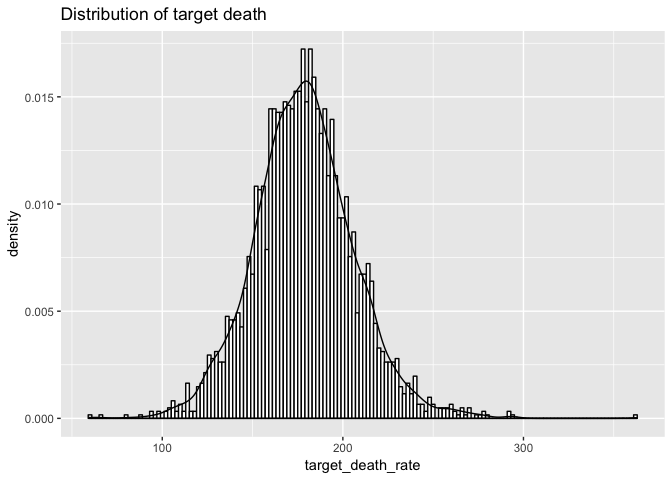
\includegraphics{p8130_final_project_files/figure-latex/unnamed-chunk-2-1.pdf}

\begin{Shaded}
\begin{Highlighting}[]
\CommentTok{#Make a histogram set to show the normal distribution of the variables to decide whether transformation is required. }
\NormalTok{cancer_s }\OperatorTok
\StringTok{  }\NormalTok{dplyr}\OperatorTok{::}\KeywordTok{select}\NormalTok{(}\OperatorTok{-}\NormalTok{age_cat) }\OperatorTok
\StringTok{  }\KeywordTok{gather}\NormalTok{(measure, value) }\OperatorTok
\StringTok{  }\KeywordTok{ggplot}\NormalTok{(}\KeywordTok{aes}\NormalTok{(value)) }\OperatorTok{+}
\StringTok{  }\KeywordTok{facet_wrap}\NormalTok{(. }\OperatorTok{~}\StringTok{ }\NormalTok{measure, }\DataTypeTok{scales =} \StringTok{"free"}\NormalTok{) }\OperatorTok{+}
\StringTok{  }\KeywordTok{geom_histogram}\NormalTok{()}
\end{Highlighting}
\end{Shaded}

\begin{verbatim}
## `stat_bin()` using `bins = 30`. Pick better value with `binwidth`.
\end{verbatim}

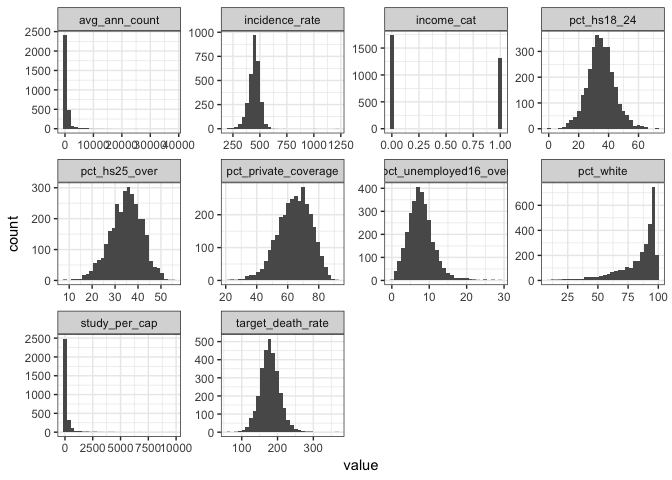
\includegraphics{p8130_final_project_files/figure-latex/unnamed-chunk-2-2.pdf}

\begin{Shaded}
\begin{Highlighting}[]
\CommentTok{#Find the significant variables in each number of parameters. Used as a reference for later removal of variables. }
\NormalTok{criterion_subset =}\StringTok{ }\KeywordTok{regsubsets}\NormalTok{(target_death_rate }\OperatorTok{~}\StringTok{ }\NormalTok{., }\DataTypeTok{data =}\NormalTok{ cancer_s, }\DataTypeTok{nvmax =} \DecValTok{34}\NormalTok{)}
\NormalTok{   (}\DataTypeTok{rs =} \KeywordTok{summary}\NormalTok{(criterion_subset))}
\end{Highlighting}
\end{Shaded}

\begin{verbatim}
## Subset selection object
## Call: regsubsets.formula(target_death_rate ~ ., data = cancer_s, nvmax = 34)
## 8 Variables  (and intercept)
##                       Forced in Forced out
## avg_ann_count             FALSE      FALSE
## incidence_rate            FALSE      FALSE
## pct_unemployed16_over     FALSE      FALSE
## age_cat                   FALSE      FALSE
## pct_private_coverage      FALSE      FALSE
## pct_white                 FALSE      FALSE
## pct_hs25_over             FALSE      FALSE
## pct_hs18_24               FALSE      FALSE
## 1 subsets of each size up to 8
## Selection Algorithm: exhaustive
##          avg_ann_count incidence_rate pct_unemployed16_over age_cat
## 1  ( 1 ) " "           "*"            " "                   " "    
## 2  ( 1 ) " "           "*"            " "                   " "    
## 3  ( 1 ) " "           "*"            " "                   " "    
## 4  ( 1 ) " "           "*"            "*"                   " "    
## 5  ( 1 ) " "           "*"            "*"                   "*"    
## 6  ( 1 ) "*"           "*"            "*"                   "*"    
## 7  ( 1 ) "*"           "*"            "*"                   "*"    
## 8  ( 1 ) "*"           "*"            "*"                   "*"    
##          pct_private_coverage pct_white pct_hs25_over pct_hs18_24
## 1  ( 1 ) " "                  " "       " "           " "        
## 2  ( 1 ) "*"                  " "       " "           " "        
## 3  ( 1 ) "*"                  " "       "*"           " "        
## 4  ( 1 ) "*"                  " "       "*"           " "        
## 5  ( 1 ) "*"                  " "       "*"           " "        
## 6  ( 1 ) "*"                  " "       "*"           " "        
## 7  ( 1 ) "*"                  " "       "*"           "*"        
## 8  ( 1 ) "*"                  "*"       "*"           "*"
\end{verbatim}

\begin{Shaded}
\begin{Highlighting}[]
\KeywordTok{par}\NormalTok{(}\DataTypeTok{mar =} \KeywordTok{c}\NormalTok{(}\DecValTok{4}\NormalTok{,}\DecValTok{4}\NormalTok{,}\DecValTok{1}\NormalTok{,}\DecValTok{1}\NormalTok{))}
\KeywordTok{par}\NormalTok{(}\DataTypeTok{mfrow =} \KeywordTok{c}\NormalTok{(}\DecValTok{1}\NormalTok{,}\DecValTok{2}\NormalTok{))}

\CommentTok{#Only when the p equals to 9, Cp=8.76 < Parameter. As a result, we decide that the number of predictors would be 9-1 = 8 or 10-1 = 9. So we look back to the significance table and we found that only the study_per_cap is not significant and we decided to remove it. }

\KeywordTok{plot}\NormalTok{(}\DecValTok{2}\OperatorTok{:}\DecValTok{9}\NormalTok{, rs}\OperatorTok{$}\NormalTok{cp, }\DataTypeTok{xlab =} \StringTok{"No of parameters"}\NormalTok{, }\DataTypeTok{ylab =} \StringTok{"Cp Statistic"}\NormalTok{)}
\KeywordTok{abline}\NormalTok{(}\DecValTok{0}\NormalTok{,}\DecValTok{1}\NormalTok{)}

\CommentTok{#And at parameter equals to 9, the adjusted r square value is highest. }
\KeywordTok{plot}\NormalTok{(}\DecValTok{2}\OperatorTok{:}\DecValTok{9}\NormalTok{, rs}\OperatorTok{$}\NormalTok{adjr2, }\DataTypeTok{xlab =} \StringTok{"No of parameters"}\NormalTok{, }\DataTypeTok{ylab =} \StringTok{"Adj R2"}\NormalTok{)}
\end{Highlighting}
\end{Shaded}

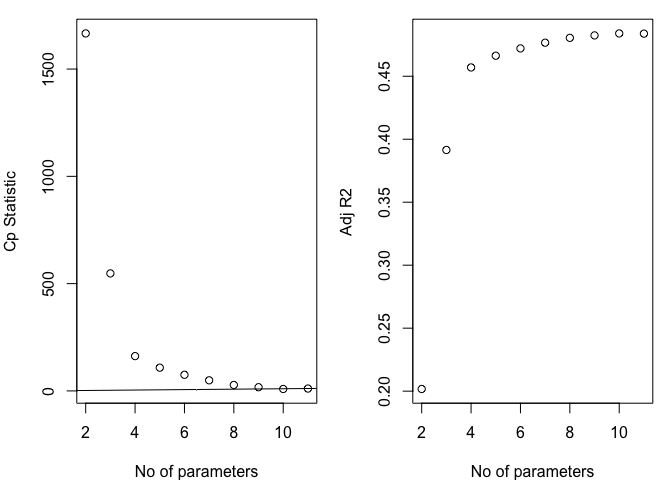
\includegraphics{p8130_final_project_files/figure-latex/unnamed-chunk-2-3.pdf}

\begin{Shaded}
\begin{Highlighting}[]
\CommentTok{#So we decide this is our final model. }
\NormalTok{cancer_lm =}\StringTok{ }\KeywordTok{lm}\NormalTok{(target_death_rate }\OperatorTok{~}\StringTok{ }\NormalTok{., }\DataTypeTok{data =}\NormalTok{ cancer_s)}
\KeywordTok{summary}\NormalTok{(cancer_lm)}
\end{Highlighting}
\end{Shaded}

\begin{verbatim}
## 
## Call:
## lm(formula = target_death_rate ~ ., data = cancer_s)
## 
## Residuals:
##      Min       1Q   Median       3Q      Max 
## -106.719  -11.851    0.029   11.195  138.436 
## 
## Coefficients:
##                         Estimate Std. Error t value Pr(>|t|)    
## (Intercept)           83.6354002  5.1423568  16.264  < 2e-16 ***
## avg_ann_count         -0.0012182  0.0002744  -4.440 9.31e-06 ***
## incidence_rate         0.2190342  0.0070103  31.244  < 2e-16 ***
## pct_unemployed16_over  0.8993821  0.1472475   6.108 1.14e-09 ***
## age_cat               -5.6381097  0.9655331  -5.839 5.79e-09 ***
## pct_private_coverage  -0.6706928  0.0489349 -13.706  < 2e-16 ***
## pct_white             -0.0801211  0.0280270  -2.859  0.00428 ** 
## pct_hs25_over          1.0065584  0.0627715  16.035  < 2e-16 ***
## pct_hs18_24            0.1825604  0.0455351   4.009 6.24e-05 ***
## ---
## Signif. codes:  0 '***' 0.001 '**' 0.01 '*' 0.05 '.' 0.1 ' ' 1
## 
## Residual standard error: 20.04 on 3038 degrees of freedom
## Multiple R-squared:  0.4802, Adjusted R-squared:  0.4788 
## F-statistic: 350.8 on 8 and 3038 DF,  p-value: < 2.2e-16
\end{verbatim}

\subsubsection{Model Diagnostic}\label{model-diagnostic}

\begin{Shaded}
\begin{Highlighting}[]
\CommentTok{#Add the row names for the data set using the geography column. }
\CommentTok{#Apply the model we built. }
\NormalTok{cancer_lm =}\StringTok{ }\KeywordTok{lm}\NormalTok{(target_death_rate }\OperatorTok{~}\StringTok{ }\NormalTok{., }\DataTypeTok{data =}\NormalTok{ cancer_s)}

\NormalTok{## outlier in Y-Look at the studendized ourliers}
\NormalTok{stu_res =}\StringTok{ }\KeywordTok{rstandard}\NormalTok{(cancer_lm)}
\NormalTok{outliers_y =}\StringTok{ }\NormalTok{stu_res[}\KeywordTok{abs}\NormalTok{(stu_res) }\OperatorTok{>}\StringTok{ }\FloatTok{2.5}\NormalTok{]}

\CommentTok{#Make four plots to show whether the assumptions are met. }
\KeywordTok{par}\NormalTok{(}\DataTypeTok{mfrow =} \KeywordTok{c}\NormalTok{(}\DecValTok{2}\NormalTok{,}\DecValTok{2}\NormalTok{))}
\KeywordTok{plot}\NormalTok{(cancer_lm)}
\end{Highlighting}
\end{Shaded}

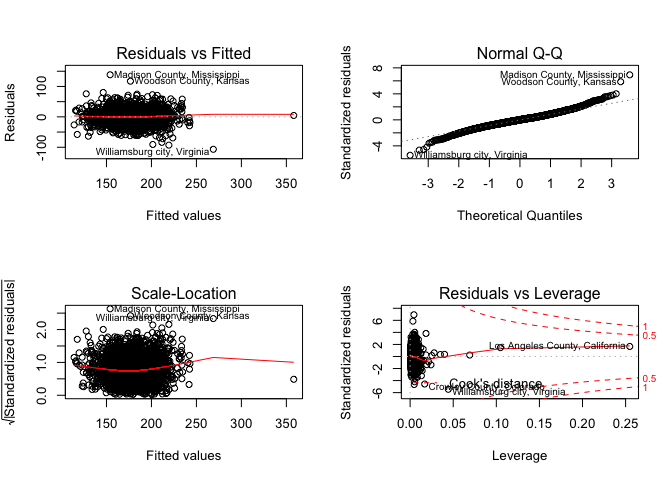
\includegraphics{p8130_final_project_files/figure-latex/unnamed-chunk-3-1.pdf}

\begin{Shaded}
\begin{Highlighting}[]
\CommentTok{# 1000 might be an influential outlier. }
\NormalTok{lev =}\StringTok{ }\KeywordTok{hatvalues}\NormalTok{(cancer_lm)}
\NormalTok{lev[lev }\OperatorTok{>}\StringTok{ }\FloatTok{0.2}\NormalTok{]}
\end{Highlighting}
\end{Shaded}

\begin{verbatim}
## Los Angeles County, California 
##                      0.2548022
\end{verbatim}

\begin{Shaded}
\begin{Highlighting}[]
\CommentTok{#a = cancer_data_analysis[-1000,]}

\CommentTok{#Calculate the DIFFITS to determine the outliers. }
\NormalTok{diffits_data =}\StringTok{ }\KeywordTok{dffits}\NormalTok{(cancer_lm) }\OperatorTok
\StringTok{  }\KeywordTok{data.frame}\NormalTok{()}

\KeywordTok{colnames}\NormalTok{(diffits_data) =}\StringTok{ }\KeywordTok{c}\NormalTok{(}\StringTok{"diffit"}\NormalTok{)}

\NormalTok{diffits_outlier =}\StringTok{ }\NormalTok{diffits_data }\OperatorTok
\StringTok{  }\KeywordTok{filter}\NormalTok{(diffit }\OperatorTok{>}\StringTok{ }\DecValTok{2}\OperatorTok{*}\KeywordTok{sqrt}\NormalTok{(}\DecValTok{8}\OperatorTok{/}\DecValTok{3047}\NormalTok{))}

\CommentTok{#not influential outlier change in coef < 6%---decide to keep all obes}
\NormalTok{cancer_s }\OperatorTok\StringTok{ }
\StringTok{  }\KeywordTok{filter}\NormalTok{(}\OperatorTok{!}\NormalTok{(}\KeywordTok{row.names}\NormalTok{(cancer_s) }\OperatorTok\StringTok{ }\KeywordTok{c}\NormalTok{(}\StringTok{"Williamsburg city, Virginia"}\NormalTok{, }\StringTok{"Madison County, Mississippi"}\NormalTok{, }\StringTok{"Woodson County, Kansas"}\NormalTok{, }\StringTok{"Aleutians West Census Area, Alaska"}\NormalTok{, }\StringTok{"Los Angeles County, California"}\NormalTok{))) }\OperatorTok\StringTok{ }
\StringTok{  }\KeywordTok{lm}\NormalTok{(target_death_rate }\OperatorTok{~}\StringTok{ }\NormalTok{., }\DataTypeTok{data=}\NormalTok{.) }\OperatorTok\StringTok{ }
\StringTok{  }\KeywordTok{summary}\NormalTok{()}
\end{Highlighting}
\end{Shaded}

\begin{verbatim}
## 
## Call:
## lm(formula = target_death_rate ~ ., data = .)
## 
## Residuals:
##    Min     1Q Median     3Q    Max 
## -94.26 -11.90   0.06  11.16  81.74 
## 
## Coefficients:
##                         Estimate Std. Error t value Pr(>|t|)    
## (Intercept)           79.5340895  5.0576987  15.725  < 2e-16 ***
## avg_ann_count         -0.0015694  0.0003114  -5.039 4.95e-07 ***
## incidence_rate         0.2291456  0.0070425  32.537  < 2e-16 ***
## pct_unemployed16_over  0.9512827  0.1443813   6.589 5.21e-11 ***
## age_cat               -5.7691627  0.9460907  -6.098 1.21e-09 ***
## pct_private_coverage  -0.6748353  0.0480761 -14.037  < 2e-16 ***
## pct_white             -0.0654012  0.0275992  -2.370 0.017866 *  
## pct_hs25_over          0.9794635  0.0619827  15.802  < 2e-16 ***
## pct_hs18_24            0.1622660  0.0446564   3.634 0.000284 ***
## ---
## Signif. codes:  0 '***' 0.001 '**' 0.01 '*' 0.05 '.' 0.1 ' ' 1
## 
## Residual standard error: 19.62 on 3033 degrees of freedom
## Multiple R-squared:  0.4965, Adjusted R-squared:  0.4951 
## F-statistic: 373.8 on 8 and 3033 DF,  p-value: < 2.2e-16
\end{verbatim}

\section{Cross-Validation}\label{cross-validation}

\begin{Shaded}
\begin{Highlighting}[]
\CommentTok{# CV for our selected variables}
\NormalTok{data_train =}\StringTok{ }\KeywordTok{trainControl}\NormalTok{(}\DataTypeTok{method =} \StringTok{"repeatedcv"}\NormalTok{, }\DataTypeTok{number =} \DecValTok{10}\NormalTok{, }\DataTypeTok{repeats =} \DecValTok{10}\NormalTok{)}
\CommentTok{# Fit the 4-variables model that we discussed in previous lectures}
\NormalTok{model_caret <-}\StringTok{ }\KeywordTok{train}\NormalTok{(target_death_rate }\OperatorTok{~}\StringTok{ }\NormalTok{avg_ann_count }\OperatorTok{+}\StringTok{ }\NormalTok{incidence_rate }\OperatorTok{+}\StringTok{ }\NormalTok{pct_unemployed16_over }\OperatorTok{+}\StringTok{ }\NormalTok{age_cat }\OperatorTok{+}\StringTok{ }\NormalTok{pct_private_coverage }\OperatorTok{+}\StringTok{ }\NormalTok{pct_white }\OperatorTok{+}\StringTok{ }\NormalTok{pct_hs25_over }\OperatorTok{+}\StringTok{ }\NormalTok{pct_hs18_}\DecValTok{24}\NormalTok{, }\DataTypeTok{data =}\NormalTok{ cancer_data_analysis,}
                   \DataTypeTok{trControl=}\NormalTok{data_train,}
                   \DataTypeTok{method=}\StringTok{'lm'}\NormalTok{,}
                   \DataTypeTok{na.action=}\NormalTok{na.pass)}
\NormalTok{model_caret}
\end{Highlighting}
\end{Shaded}

\begin{verbatim}
## Linear Regression 
## 
## 3047 samples
##    8 predictor
## 
## No pre-processing
## Resampling: Cross-Validated (10 fold, repeated 10 times) 
## Summary of sample sizes: 2742, 2743, 2741, 2743, 2741, 2741, ... 
## Resampling results:
## 
##   RMSE      Rsquared   MAE    
##   20.06379  0.4773481  14.9672
## 
## Tuning parameter 'intercept' was held constant at a value of TRUE
\end{verbatim}

\begin{Shaded}
\begin{Highlighting}[]
\CommentTok{# CV for more variables (including unselected)}
\NormalTok{data_train_}\DecValTok{2}\NormalTok{ =}\StringTok{ }\KeywordTok{trainControl}\NormalTok{(}\DataTypeTok{method =} \StringTok{"repeatedcv"}\NormalTok{, }\DataTypeTok{number =} \DecValTok{10}\NormalTok{, }\DataTypeTok{repeats =} \DecValTok{10}\NormalTok{)}
\NormalTok{model_caret_}\DecValTok{2}\NormalTok{ =}\StringTok{ }\KeywordTok{train}\NormalTok{(target_death_rate }\OperatorTok{~}\StringTok{ }\NormalTok{incidence_rate }\OperatorTok{+}\StringTok{ }\NormalTok{poverty_percent }\OperatorTok{+}\StringTok{ }\NormalTok{median_age_female }
                    \OperatorTok{+}\StringTok{ }\NormalTok{percent_married }\OperatorTok{+}\StringTok{ }\NormalTok{pct_hs18_}\DecValTok{24} \OperatorTok{+}\StringTok{ }\NormalTok{pct_hs25_over }\OperatorTok{+}\StringTok{ }\NormalTok{pct_bach_deg25_over }
                    \OperatorTok{+}\StringTok{ }\NormalTok{pct_unemployed16_over }\OperatorTok{+}\StringTok{ }\NormalTok{pct_private_coverage }\OperatorTok{+}\StringTok{ }\NormalTok{pct_emp_priv_coverage }
                    \OperatorTok{+}\StringTok{ }\NormalTok{pct_public_coverage }\OperatorTok{+}\StringTok{ }\NormalTok{pct_white }\OperatorTok{+}\StringTok{ }\NormalTok{pct_black }\OperatorTok{+}\StringTok{ }\NormalTok{pct_other_race }\OperatorTok{+}\StringTok{ }\NormalTok{birth_rate, }
                    \DataTypeTok{data =}\NormalTok{ cancer_data_analysis,}
                    \DataTypeTok{trControl=}\NormalTok{data_train_}\DecValTok{2}\NormalTok{,}
                    \DataTypeTok{method=}\StringTok{'lm'}\NormalTok{,}
                    \DataTypeTok{na.action=}\NormalTok{na.pass)}

\NormalTok{RMSE =}\StringTok{ }\KeywordTok{mean}\NormalTok{(model_caret_}\DecValTok{2}\OperatorTok{$}\NormalTok{resample}\OperatorTok{$}\NormalTok{RMSE)}
\NormalTok{RMSE}
\end{Highlighting}
\end{Shaded}

\begin{verbatim}
## [1] 19.66037
\end{verbatim}

\section{Bootstrap}\label{bootstrap}

\begin{Shaded}
\begin{Highlighting}[]
\NormalTok{boot.fn<-}\ControlFlowTok{function}\NormalTok{(data, index)\{}
    \KeywordTok{return}\NormalTok{(}\KeywordTok{coef}\NormalTok{(}\KeywordTok{lm}\NormalTok{(target_death_rate }\OperatorTok{~}\StringTok{ }\NormalTok{., }\DataTypeTok{data =}\NormalTok{ data, }\DataTypeTok{subset=}\NormalTok{index)))}
\NormalTok{\}}

\NormalTok{results =}\StringTok{ }\KeywordTok{boot}\NormalTok{(cancer_s, boot.fn, }\DecValTok{10000}\NormalTok{)}
\KeywordTok{rmse}\NormalTok{(cancer_lm, cancer_s)}
\end{Highlighting}
\end{Shaded}

\begin{verbatim}
## [1] 20.00552
\end{verbatim}

\begin{Shaded}
\begin{Highlighting}[]
\KeywordTok{plot}\NormalTok{(results, }\DataTypeTok{index =} \DecValTok{1}\NormalTok{)}
\end{Highlighting}
\end{Shaded}

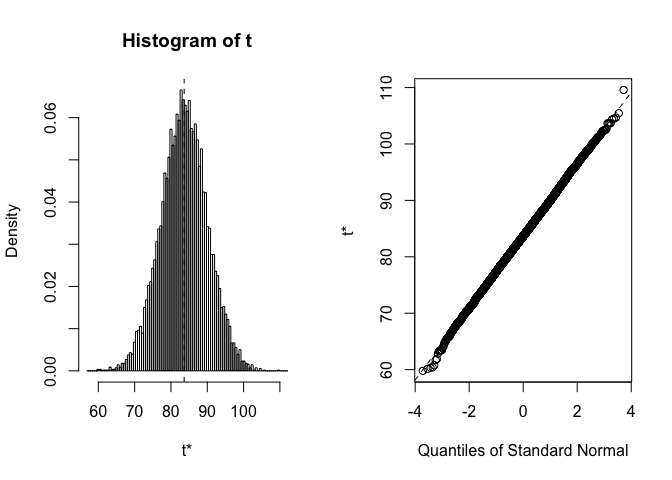
\includegraphics{p8130_final_project_files/figure-latex/bootstrap-1.pdf}

\begin{Shaded}
\begin{Highlighting}[]
\CommentTok{#results$t[ ,1]}

\CommentTok{#results_raw = boot(cancer_data_analysis, boot.fn, 10000)}
\CommentTok{#cancer_overall = lm(target_death_rate ~ ., data = cancer_data_analysis)}
\CommentTok{#rmse(cancer_overall, cancer_data_analysis)}
\CommentTok{#plot(results_raw, index = 1)}
\end{Highlighting}
\end{Shaded}

\begin{Shaded}
\begin{Highlighting}[]
\CommentTok{#install.packages("parcor")}
\KeywordTok{library}\NormalTok{(parcor)}
\end{Highlighting}
\end{Shaded}

\begin{verbatim}
## Loading required package: MASS
\end{verbatim}

\begin{verbatim}
## 
## Attaching package: 'MASS'
\end{verbatim}

\begin{verbatim}
## The following object is masked from 'package:dplyr':
## 
##     select
\end{verbatim}

\begin{verbatim}
## Loading required package: glmnet
\end{verbatim}

\begin{verbatim}
## Loading required package: Matrix
\end{verbatim}

\begin{verbatim}
## 
## Attaching package: 'Matrix'
\end{verbatim}

\begin{verbatim}
## The following object is masked from 'package:tidyr':
## 
##     expand
\end{verbatim}

\begin{verbatim}
## Loading required package: foreach
\end{verbatim}

\begin{verbatim}
## 
## Attaching package: 'foreach'
\end{verbatim}

\begin{verbatim}
## The following objects are masked from 'package:purrr':
## 
##     accumulate, when
\end{verbatim}

\begin{verbatim}
## Loaded glmnet 2.0-16
\end{verbatim}

\begin{verbatim}
## Loading required package: ppls
\end{verbatim}

\begin{verbatim}
## Loading required package: splines
\end{verbatim}

\begin{verbatim}
## Loading required package: Epi
\end{verbatim}

\begin{verbatim}
## Loading required package: GeneNet
\end{verbatim}

\begin{verbatim}
## Loading required package: corpcor
\end{verbatim}

\begin{verbatim}
## Loading required package: longitudinal
\end{verbatim}

\begin{verbatim}
## Loading required package: fdrtool
\end{verbatim}

\begin{Shaded}
\begin{Highlighting}[]
\KeywordTok{library}\NormalTok{(MASS)}
\KeywordTok{library}\NormalTok{(glmnet)}
\KeywordTok{library}\NormalTok{(reshape2)}
\end{Highlighting}
\end{Shaded}

\begin{verbatim}
## 
## Attaching package: 'reshape2'
\end{verbatim}

\begin{verbatim}
## The following object is masked from 'package:tidyr':
## 
##     smiths
\end{verbatim}

\begin{Shaded}
\begin{Highlighting}[]
\CommentTok{# Start with the full model}
\NormalTok{mult.fit <-}\StringTok{ }\KeywordTok{lm}\NormalTok{(target_death_rate }\OperatorTok{~}\StringTok{ }\NormalTok{., }\DataTypeTok{data=}\NormalTok{cancer_s)}
\KeywordTok{summary}\NormalTok{(mult.fit)}
\end{Highlighting}
\end{Shaded}

\begin{verbatim}
## 
## Call:
## lm(formula = target_death_rate ~ ., data = cancer_s)
## 
## Residuals:
##      Min       1Q   Median       3Q      Max 
## -106.719  -11.851    0.029   11.195  138.436 
## 
## Coefficients:
##                         Estimate Std. Error t value Pr(>|t|)    
## (Intercept)           83.6354002  5.1423568  16.264  < 2e-16 ***
## avg_ann_count         -0.0012182  0.0002744  -4.440 9.31e-06 ***
## incidence_rate         0.2190342  0.0070103  31.244  < 2e-16 ***
## pct_unemployed16_over  0.8993821  0.1472475   6.108 1.14e-09 ***
## age_cat               -5.6381097  0.9655331  -5.839 5.79e-09 ***
## pct_private_coverage  -0.6706928  0.0489349 -13.706  < 2e-16 ***
## pct_white             -0.0801211  0.0280270  -2.859  0.00428 ** 
## pct_hs25_over          1.0065584  0.0627715  16.035  < 2e-16 ***
## pct_hs18_24            0.1825604  0.0455351   4.009 6.24e-05 ***
## ---
## Signif. codes:  0 '***' 0.001 '**' 0.01 '*' 0.05 '.' 0.1 ' ' 1
## 
## Residual standard error: 20.04 on 3038 degrees of freedom
## Multiple R-squared:  0.4802, Adjusted R-squared:  0.4788 
## F-statistic: 350.8 on 8 and 3038 DF,  p-value: < 2.2e-16
\end{verbatim}

\begin{Shaded}
\begin{Highlighting}[]
\CommentTok{#Ridge Regression}
\NormalTok{ridge1 <-}\StringTok{ }\KeywordTok{lm.ridge}\NormalTok{(target_death_rate }\OperatorTok{~}\NormalTok{., }\DataTypeTok{data=}\NormalTok{cancer_s)}
\NormalTok{ridge1}
\end{Highlighting}
\end{Shaded}

\begin{verbatim}
##                               avg_ann_count        incidence_rate 
##          83.635400234          -0.001218187           0.219034158 
## pct_unemployed16_over               age_cat  pct_private_coverage 
##           0.899382075          -5.638109741          -0.670692834 
##             pct_white         pct_hs25_over           pct_hs18_24 
##          -0.080121146           1.006558361           0.182560358
\end{verbatim}

\begin{Shaded}
\begin{Highlighting}[]
\CommentTok{# Compare the LS and Ridge coefficients.}
\CommentTok{# No difference because the default value for lambda (tunning parameter) is set to 0 by default.}
\KeywordTok{coef}\NormalTok{(ridge1)}
\end{Highlighting}
\end{Shaded}

\begin{verbatim}
##                               avg_ann_count        incidence_rate 
##          83.635400234          -0.001218187           0.219034158 
## pct_unemployed16_over               age_cat  pct_private_coverage 
##           0.899382075          -5.638109741          -0.670692834 
##             pct_white         pct_hs25_over           pct_hs18_24 
##          -0.080121146           1.006558361           0.182560358
\end{verbatim}

\begin{Shaded}
\begin{Highlighting}[]
\KeywordTok{coef}\NormalTok{(mult.fit)}
\end{Highlighting}
\end{Shaded}

\begin{verbatim}
##           (Intercept)         avg_ann_count        incidence_rate 
##          83.635400234          -0.001218187           0.219034158 
## pct_unemployed16_over               age_cat  pct_private_coverage 
##           0.899382075          -5.638109741          -0.670692834 
##             pct_white         pct_hs25_over           pct_hs18_24 
##          -0.080121146           1.006558361           0.182560358
\end{verbatim}

\begin{Shaded}
\begin{Highlighting}[]
\CommentTok{# Try a grid of values for lambda: from 10^-2 to 10^5}

\NormalTok{grid <-}\StringTok{ }\DecValTok{10}\OperatorTok{^}\KeywordTok{seq}\NormalTok{(}\DecValTok{5}\NormalTok{,}\OperatorTok{-}\DecValTok{2}\NormalTok{, }\DataTypeTok{length=}\DecValTok{100}\NormalTok{)}


\CommentTok{# Matrix of 100X8 containing coefficients for all 100 values of lambda}
\NormalTok{ridge2 <-}\StringTok{ }\KeywordTok{lm.ridge}\NormalTok{(target_death_rate }\OperatorTok{~}\NormalTok{., }\DataTypeTok{data=}\NormalTok{cancer_s, }\DataTypeTok{lambda=}\NormalTok{grid)}
\KeywordTok{dim}\NormalTok{(}\KeywordTok{coef}\NormalTok{(ridge2))}
\end{Highlighting}
\end{Shaded}

\begin{verbatim}
## [1] 100   9
\end{verbatim}

\begin{Shaded}
\begin{Highlighting}[]
\NormalTok{######################################################}
\CommentTok{#            Use function glmnet()                   #}
\NormalTok{######################################################}

\NormalTok{cancer_df =}\StringTok{ }\KeywordTok{data.frame}\NormalTok{(cancer_s)}
\NormalTok{Y <-}\StringTok{ }\NormalTok{cancer_df[,}\DecValTok{1}\NormalTok{]}
\NormalTok{X <-}\StringTok{ }\KeywordTok{as.matrix}\NormalTok{(cancer_df[,}\OperatorTok{-}\DecValTok{1}\NormalTok{])}

\CommentTok{# Penalty term: alpha; Ridge alpha=0 (default); Lasso alpha=1 (default)}
\NormalTok{ridge3<-}\KeywordTok{glmnet}\NormalTok{(X, Y, }\DataTypeTok{alpha =} \DecValTok{0}\NormalTok{, }\DataTypeTok{lambda =}\NormalTok{ grid)}
\KeywordTok{dim}\NormalTok{(}\KeywordTok{coef}\NormalTok{(ridge3))}
\end{Highlighting}
\end{Shaded}

\begin{verbatim}
## [1]   9 100
\end{verbatim}

\begin{Shaded}
\begin{Highlighting}[]
\CommentTok{# Look at lambda and the coeff estimates on position 50}
\NormalTok{ridge3}\OperatorTok{$}\NormalTok{lambda[}\DecValTok{50}\NormalTok{]}
\end{Highlighting}
\end{Shaded}

\begin{verbatim}
## [1] 34.30469
\end{verbatim}

\begin{Shaded}
\begin{Highlighting}[]
\KeywordTok{coef}\NormalTok{(ridge3)[,}\DecValTok{50}\NormalTok{]}
\end{Highlighting}
\end{Shaded}

\begin{verbatim}
##           (Intercept)         avg_ann_count        incidence_rate 
##         128.467553728          -0.000824085           0.098208440 
## pct_unemployed16_over               age_cat  pct_private_coverage 
##           0.853927930          -3.016570749          -0.308865451 
##             pct_white         pct_hs25_over           pct_hs18_24 
##          -0.073402548           0.555109837           0.206267931
\end{verbatim}

\begin{Shaded}
\begin{Highlighting}[]
\CommentTok{# L2 norm for Ridge}
\CommentTok{# sqrt(sum(coef(ridge3)[-1,50]^2))}
\CommentTok{#Choice of lambda: Cross Validation (CV)}
\CommentTok{# Choose the training sample: 50:50}

\KeywordTok{set.seed}\NormalTok{(}\DecValTok{1}\NormalTok{)}
\NormalTok{train<-}\KeywordTok{sample}\NormalTok{(}\DecValTok{1}\OperatorTok{:}\KeywordTok{nrow}\NormalTok{(X),}\KeywordTok{nrow}\NormalTok{(X)}\OperatorTok{/}\DecValTok{2}\NormalTok{)}
\NormalTok{test<-(}\OperatorTok{-}\NormalTok{train)}
\NormalTok{Y.test<-Y[test]}

\CommentTok{# Use build-in CV function; performs a 10-fold validation by default}
\CommentTok{# glmnet() generates it's own lambda sequence}

\KeywordTok{set.seed}\NormalTok{(}\DecValTok{2}\NormalTok{)}
\NormalTok{cv.out<-}\KeywordTok{cv.glmnet}\NormalTok{(X[train,],Y[train], }\DataTypeTok{alpha=}\DecValTok{0}\NormalTok{)}
\KeywordTok{plot}\NormalTok{(cv.out)}
\end{Highlighting}
\end{Shaded}

\includegraphics{p8130_final_project_files/figure-latex/ridge\&lasso-1.pdf}

\begin{Shaded}
\begin{Highlighting}[]
\CommentTok{# cv.glmnet() object contains the mean cross-validation error (cvm),}
\CommentTok{# lambda min that gives the minimum cvm, etc.}
\NormalTok{cv.out}
\end{Highlighting}
\end{Shaded}

\begin{verbatim}
## $lambda
##  [1] 13072.277547 11910.972439 10852.834477  9888.698574  9010.213848
##  [6]  8209.771284  7480.437831  6815.896351  6210.390905  5658.676894
## [11]  5155.975636  4697.932971  4280.581554  3900.306487  3553.814009
## [16]  3238.102967  2950.438824  2688.329971  2449.506146  2231.898771
## [21]  2033.623036  1852.961571  1688.349572  1538.361249  1401.697476
## [26]  1277.174536  1163.713870  1060.332737   966.135699   880.306867
## [31]   802.102831   730.846226   665.919862   606.761377   552.858368
## [36]   503.743955   458.992730   418.217081   381.063828   347.211168
## [41]   316.365885   288.260812   262.652516   239.319190   218.058733
## [46]   198.686996   181.036191   164.953435   150.299426   136.947239
## [51]   124.781224   113.696004   103.595564    94.392420    86.006858
## [56]    78.366245    71.404404    65.061034    59.281191    54.014813
## [61]    49.216286    44.844047    40.860225    37.230316    33.922877
## [66]    30.909262    28.163368    25.661412    23.381723    21.304555
## [71]    19.411917    17.687416    16.116115    14.684404    13.379882
## [76]    12.191250    11.108213    10.121390     9.222233     8.402956
## [81]     7.656460     6.976281     6.356528     5.791831     5.277301
## [86]     4.808480     4.381308     3.992085     3.637439     3.314299
## [91]     3.019866     2.751589     2.507146     2.284418     2.081476
## [96]     1.896564     1.728078     1.574560     1.434681
## 
## $cvm
##  [1] 802.2753 799.8879 799.1164 798.7760 798.4030 797.9943 797.5466
##  [8] 797.0561 796.5191 795.9310 795.2873 794.5828 793.8120 792.9689
## [15] 792.0471 791.0395 789.9386 788.7363 787.4239 785.9919 784.4304
## [22] 782.7287 780.8754 778.8585 776.6653 774.2823 771.6956 768.8907
## [29] 765.8524 762.5652 759.0135 755.1813 751.0526 746.6120 741.8442
## [36] 736.7350 731.2710 725.4406 719.2338 712.6430 705.6633 698.2930
## [43] 690.5340 682.3921 673.8776 665.0058 655.7965 646.2750 636.4716
## [50] 626.4216 616.1652 605.7469 595.2150 584.6209 574.0183 563.4622
## [57] 553.0078 542.7097 532.6207 522.7905 513.2654 504.0868 495.2911
## [64] 486.9088 478.9644 471.4759 464.4552 457.9083 451.8353 446.2306
## [71] 441.0844 436.3824 432.1071 428.2381 424.7527 421.6269 418.8358
## [78] 416.3541 414.1564 412.2180 410.5149 409.0243 407.7244 406.5950
## [85] 405.6170 404.7733 404.0478 403.4261 402.8951 402.4432 402.0598
## [92] 401.7358 401.4628 401.2337 401.0421 400.8824 400.7500 400.6409
## [99] 400.5516
## 
## $cvsd
##  [1] 32.40974 32.29767 32.17703 32.16394 32.14959 32.13386 32.11662
##  [8] 32.09773 32.07703 32.05434 32.02950 32.00229 31.97250 31.93988
## [15] 31.90419 31.86513 31.82241 31.77569 31.72463 31.66884 31.60791
## [22] 31.54139 31.46881 31.38966 31.30341 31.20947 31.10725 30.99610
## [29] 30.87535 30.74431 30.60224 30.44840 30.28203 30.10237 29.90866
## [36] 29.70015 29.47612 29.23592 28.97895 28.70470 28.41277 28.10295
## [43] 27.77515 27.42952 27.06645 26.68663 26.29103 25.88097 25.45816
## [50] 25.02466 24.58294 24.13585 23.68661 23.23875 22.79605 22.36251
## [57] 21.94217 21.53907 21.15707 20.79972 20.47018 20.17102 19.90420
## [64] 19.67093 19.47170 19.30626 19.17365 19.07228 18.99999 18.95459
## [71] 18.93322 18.93302 18.95108 18.98456 19.03076 19.08716 19.15146
## [78] 19.22160 19.29579 19.37246 19.45029 19.52817 19.60519 19.68063
## [85] 19.75390 19.82456 19.89230 19.95690 20.01820 20.07616 20.13074
## [92] 20.18198 20.22995 20.27474 20.31647 20.35526 20.39125 20.42465
## [99] 20.45557
## 
## $cvup
##  [1] 834.6851 832.1855 831.2934 830.9399 830.5526 830.1282 829.6632
##  [8] 829.1539 828.5961 827.9853 827.3168 826.5850 825.7845 824.9088
## [15] 823.9513 822.9046 821.7610 820.5120 819.1485 817.6608 816.0383
## [22] 814.2701 812.3442 810.2482 807.9687 805.4918 802.8029 799.8868
## [29] 796.7277 793.3095 789.6157 785.6297 781.3347 776.7144 771.7529
## [36] 766.4351 760.7471 754.6765 748.2127 741.3477 734.0761 726.3960
## [43] 718.3091 709.8216 700.9441 691.6924 682.0875 672.1560 661.9298
## [50] 651.4463 640.7481 629.8827 618.9016 607.8596 596.8143 585.8247
## [57] 574.9500 564.2488 553.7777 543.5902 533.7355 524.2578 515.1953
## [64] 506.5798 498.4361 490.7821 483.6288 476.9806 470.8353 465.1852
## [71] 460.0176 455.3154 451.0582 447.2227 443.7835 440.7141 437.9873
## [78] 435.5757 433.4522 431.5904 429.9652 428.5525 427.3296 426.2756
## [85] 425.3709 424.5978 423.9401 423.3829 422.9133 422.5193 422.1906
## [92] 421.9178 421.6928 421.5084 421.3585 421.2377 421.1413 421.0656
## [99] 421.0072
## 
## $cvlo
##  [1] 769.8656 767.5902 766.9393 766.6121 766.2534 765.8604 765.4300
##  [8] 764.9584 764.4420 763.8766 763.2578 762.5805 761.8395 761.0290
## [15] 760.1429 759.1744 758.1162 756.9606 755.6993 754.3231 752.8225
## [22] 751.1873 749.4066 747.4688 745.3618 743.0728 740.5884 737.8946
## [29] 734.9770 731.8209 728.4113 724.7329 720.7706 716.5096 711.9356
## [36] 707.0348 701.7949 696.2047 690.2548 683.9383 677.2505 670.1901
## [43] 662.7588 654.9626 646.8112 638.3191 629.5055 620.3941 611.0134
## [50] 601.3970 591.5823 581.6110 571.5283 561.3821 551.2222 541.0996
## [57] 531.0656 521.1707 511.4636 501.9908 492.7952 483.9158 475.3869
## [64] 467.2379 459.4927 452.1696 445.2815 438.8360 432.8354 427.2760
## [71] 422.1511 417.4494 413.1561 409.2535 405.7219 402.5398 399.6844
## [78] 397.1325 394.8606 392.8455 391.0646 389.4961 388.1192 386.9143
## [85] 385.8631 384.9487 384.1555 383.4692 382.8769 382.3670 381.9291
## [92] 381.5538 381.2329 380.9589 380.7256 380.5272 380.3588 380.2163
## [99] 380.0961
## 
## $nzero
##  s0  s1  s2  s3  s4  s5  s6  s7  s8  s9 s10 s11 s12 s13 s14 s15 s16 s17 
##   8   8   8   8   8   8   8   8   8   8   8   8   8   8   8   8   8   8 
## s18 s19 s20 s21 s22 s23 s24 s25 s26 s27 s28 s29 s30 s31 s32 s33 s34 s35 
##   8   8   8   8   8   8   8   8   8   8   8   8   8   8   8   8   8   8 
## s36 s37 s38 s39 s40 s41 s42 s43 s44 s45 s46 s47 s48 s49 s50 s51 s52 s53 
##   8   8   8   8   8   8   8   8   8   8   8   8   8   8   8   8   8   8 
## s54 s55 s56 s57 s58 s59 s60 s61 s62 s63 s64 s65 s66 s67 s68 s69 s70 s71 
##   8   8   8   8   8   8   8   8   8   8   8   8   8   8   8   8   8   8 
## s72 s73 s74 s75 s76 s77 s78 s79 s80 s81 s82 s83 s84 s85 s86 s87 s88 s89 
##   8   8   8   8   8   8   8   8   8   8   8   8   8   8   8   8   8   8 
## s90 s91 s92 s93 s94 s95 s96 s97 s98 
##   8   8   8   8   8   8   8   8   8 
## 
## $name
##                  mse 
## "Mean-Squared Error" 
## 
## $glmnet.fit
## 
## Call:  glmnet(x = X[train, ], y = Y[train], alpha = 0) 
## 
##        Df      %Dev    Lambda
##   [1,]  8 1.718e-36 13070.000
##   [2,]  8 4.017e-03 11910.000
##   [3,]  8 4.406e-03 10850.000
##   [4,]  8 4.833e-03  9889.000
##   [5,]  8 5.300e-03  9010.000
##   [6,]  8 5.811e-03  8210.000
##   [7,]  8 6.372e-03  7480.000
##   [8,]  8 6.986e-03  6816.000
##   [9,]  8 7.659e-03  6210.000
##  [10,]  8 8.395e-03  5659.000
##  [11,]  8 9.201e-03  5156.000
##  [12,]  8 1.008e-02  4698.000
##  [13,]  8 1.105e-02  4281.000
##  [14,]  8 1.210e-02  3900.000
##  [15,]  8 1.326e-02  3554.000
##  [16,]  8 1.452e-02  3238.000
##  [17,]  8 1.590e-02  2950.000
##  [18,]  8 1.740e-02  2688.000
##  [19,]  8 1.905e-02  2450.000
##  [20,]  8 2.084e-02  2232.000
##  [21,]  8 2.280e-02  2034.000
##  [22,]  8 2.493e-02  1853.000
##  [23,]  8 2.725e-02  1688.000
##  [24,]  8 2.978e-02  1538.000
##  [25,]  8 3.252e-02  1402.000
##  [26,]  8 3.551e-02  1277.000
##  [27,]  8 3.875e-02  1164.000
##  [28,]  8 4.226e-02  1060.000
##  [29,]  8 4.607e-02   966.100
##  [30,]  8 5.019e-02   880.300
##  [31,]  8 5.464e-02   802.100
##  [32,]  8 5.944e-02   730.800
##  [33,]  8 6.461e-02   665.900
##  [34,]  8 7.018e-02   606.800
##  [35,]  8 7.615e-02   552.900
##  [36,]  8 8.256e-02   503.700
##  [37,]  8 8.940e-02   459.000
##  [38,]  8 9.671e-02   418.200
##  [39,]  8 1.045e-01   381.100
##  [40,]  8 1.128e-01   347.200
##  [41,]  8 1.215e-01   316.400
##  [42,]  8 1.308e-01   288.300
##  [43,]  8 1.405e-01   262.700
##  [44,]  8 1.507e-01   239.300
##  [45,]  8 1.614e-01   218.100
##  [46,]  8 1.725e-01   198.700
##  [47,]  8 1.841e-01   181.000
##  [48,]  8 1.960e-01   165.000
##  [49,]  8 2.083e-01   150.300
##  [50,]  8 2.209e-01   136.900
##  [51,]  8 2.338e-01   124.800
##  [52,]  8 2.469e-01   113.700
##  [53,]  8 2.601e-01   103.600
##  [54,]  8 2.735e-01    94.390
##  [55,]  8 2.868e-01    86.010
##  [56,]  8 3.001e-01    78.370
##  [57,]  8 3.132e-01    71.400
##  [58,]  8 3.262e-01    65.060
##  [59,]  8 3.389e-01    59.280
##  [60,]  8 3.512e-01    54.010
##  [61,]  8 3.632e-01    49.220
##  [62,]  8 3.748e-01    44.840
##  [63,]  8 3.859e-01    40.860
##  [64,]  8 3.965e-01    37.230
##  [65,]  8 4.065e-01    33.920
##  [66,]  8 4.160e-01    30.910
##  [67,]  8 4.248e-01    28.160
##  [68,]  8 4.331e-01    25.660
##  [69,]  8 4.408e-01    23.380
##  [70,]  8 4.479e-01    21.300
##  [71,]  8 4.545e-01    19.410
##  [72,]  8 4.604e-01    17.690
##  [73,]  8 4.659e-01    16.120
##  [74,]  8 4.708e-01    14.680
##  [75,]  8 4.753e-01    13.380
##  [76,]  8 4.793e-01    12.190
##  [77,]  8 4.829e-01    11.110
##  [78,]  8 4.861e-01    10.120
##  [79,]  8 4.890e-01     9.222
##  [80,]  8 4.915e-01     8.403
##  [81,]  8 4.937e-01     7.656
##  [82,]  8 4.957e-01     6.976
##  [83,]  8 4.974e-01     6.357
##  [84,]  8 4.989e-01     5.792
##  [85,]  8 5.002e-01     5.277
##  [86,]  8 5.013e-01     4.808
##  [87,]  8 5.023e-01     4.381
##  [88,]  8 5.031e-01     3.992
##  [89,]  8 5.039e-01     3.637
##  [90,]  8 5.045e-01     3.314
##  [91,]  8 5.050e-01     3.020
##  [92,]  8 5.055e-01     2.752
##  [93,]  8 5.059e-01     2.507
##  [94,]  8 5.062e-01     2.284
##  [95,]  8 5.065e-01     2.081
##  [96,]  8 5.068e-01     1.897
##  [97,]  8 5.070e-01     1.728
##  [98,]  8 5.071e-01     1.575
##  [99,]  8 5.073e-01     1.435
## [100,]  8 5.074e-01     1.307
## 
## $lambda.min
## [1] 1.434681
## 
## $lambda.1se
## [1] 11.10821
## 
## attr(,"class")
## [1] "cv.glmnet"
\end{verbatim}

\begin{Shaded}
\begin{Highlighting}[]
\NormalTok{best.lambda<-cv.out}\OperatorTok{$}\NormalTok{lambda.min}
\NormalTok{best.lambda}
\end{Highlighting}
\end{Shaded}

\begin{verbatim}
## [1] 1.434681
\end{verbatim}

\begin{Shaded}
\begin{Highlighting}[]
\CommentTok{# Re-fit the model with the min lambda value, look at the coeff and MSE}
\CommentTok{#ridge.pred <- predict(ridge.cv(), s = best.lambda, newx = X[test,])}

\CommentTok{#mean((ridge.pred-Y.test)^2)}

\CommentTok{# Ridge regression using all observations and 'best' lambda}
\NormalTok{ridge3<-}\KeywordTok{glmnet}\NormalTok{(X, Y, }\DataTypeTok{alpha=}\DecValTok{0}\NormalTok{, }\DataTypeTok{lambda=}\NormalTok{best.lambda)}
\NormalTok{res_ridge_ls<-}\StringTok{ }\KeywordTok{cbind}\NormalTok{(}\KeywordTok{coef}\NormalTok{(mult.fit),}\KeywordTok{coef}\NormalTok{(ridge3))}
\KeywordTok{colnames}\NormalTok{(res_ridge_ls) <-}\StringTok{ }\KeywordTok{c}\NormalTok{(}\StringTok{"LS"}\NormalTok{, }\StringTok{"Ridge"}\NormalTok{)}
\NormalTok{res_ridge_ls}
\end{Highlighting}
\end{Shaded}

\begin{verbatim}
## 9 x 2 sparse Matrix of class "dgCMatrix"
##                                 LS        Ridge
## (Intercept)           83.635400234 85.815481519
## avg_ann_count         -0.001218187 -0.001204788
## incidence_rate         0.219034158  0.207371851
## pct_unemployed16_over  0.899382075  0.964806944
## age_cat               -5.638109741 -5.448815957
## pct_private_coverage  -0.670692834 -0.619506851
## pct_white             -0.080121146 -0.082353254
## pct_hs25_over          1.006558361  0.974866524
## pct_hs18_24            0.182560358  0.196463572
\end{verbatim}

\begin{Shaded}
\begin{Highlighting}[]
\CommentTok{#Lasso regression}
\NormalTok{lasso1<-}\StringTok{ }\KeywordTok{glmnet}\NormalTok{(X[train ,],Y[train], }\DataTypeTok{alpha =}\DecValTok{1}\NormalTok{, }\DataTypeTok{lambda=}\NormalTok{grid)}


\CommentTok{# Cross-validation}
\KeywordTok{set.seed}\NormalTok{(}\DecValTok{2}\NormalTok{)}
\NormalTok{cv.out<-}\KeywordTok{cv.glmnet}\NormalTok{(X[train,],Y[train])}
\KeywordTok{plot}\NormalTok{(cv.out)}
\end{Highlighting}
\end{Shaded}

\includegraphics{p8130_final_project_files/figure-latex/ridge\&lasso-2.pdf}

\begin{Shaded}
\begin{Highlighting}[]
\NormalTok{best.lambda<-cv.out}\OperatorTok{$}\NormalTok{lambda.min}

\CommentTok{#lasso.pred=predict(lasso1,s=best.lambda,newx=X[test,])}
\CommentTok{#mean((lasso.pred-Y.test)^2)}

\CommentTok{# Fit a Lasso model with all observations with the best lambda}
\NormalTok{lasso2<-}\StringTok{ }\KeywordTok{glmnet}\NormalTok{(X, Y, }\DataTypeTok{alpha =}\DecValTok{1}\NormalTok{, }\DataTypeTok{lambda=}\NormalTok{best.lambda)}
\KeywordTok{coef}\NormalTok{(lasso2)}
\end{Highlighting}
\end{Shaded}

\begin{verbatim}
## 9 x 1 sparse Matrix of class "dgCMatrix"
##                                 s0
## (Intercept)           84.035026130
## avg_ann_count         -0.001174144
## incidence_rate         0.217942886
## pct_unemployed16_over  0.896867001
## age_cat               -5.486292003
## pct_private_coverage  -0.669473396
## pct_white             -0.076562502
## pct_hs25_over          1.002115878
## pct_hs18_24            0.177791456
\end{verbatim}

\begin{Shaded}
\begin{Highlighting}[]
\KeywordTok{coef}\NormalTok{(mult.fit)}
\end{Highlighting}
\end{Shaded}

\begin{verbatim}
##           (Intercept)         avg_ann_count        incidence_rate 
##          83.635400234          -0.001218187           0.219034158 
## pct_unemployed16_over               age_cat  pct_private_coverage 
##           0.899382075          -5.638109741          -0.670692834 
##             pct_white         pct_hs25_over           pct_hs18_24 
##          -0.080121146           1.006558361           0.182560358
\end{verbatim}

\begin{Shaded}
\begin{Highlighting}[]
\CommentTok{# Fraction of deviance explained}
\CommentTok{# Similar interpretation to R-squared: % variance explained by non-zero variables variables}
\NormalTok{lasso2}\OperatorTok{$}\NormalTok{dev.ratio}
\end{Highlighting}
\end{Shaded}

\begin{verbatim}
## [1] 0.4801328
\end{verbatim}

\begin{Shaded}
\begin{Highlighting}[]
\CommentTok{# Compare LS, Ridge and Lasso regression coefficients}
\NormalTok{res_ls_ridge_lasso<-}\StringTok{ }\KeywordTok{cbind}\NormalTok{(}\KeywordTok{coef}\NormalTok{(mult.fit),}\KeywordTok{coef}\NormalTok{(ridge3),}\KeywordTok{coef}\NormalTok{(lasso2))}
\KeywordTok{colnames}\NormalTok{(res_ls_ridge_lasso) <-}\StringTok{ }\KeywordTok{c}\NormalTok{(}\StringTok{"LS"}\NormalTok{, }\StringTok{"Ridge"}\NormalTok{,}\StringTok{"Lasso"}\NormalTok{)}
\NormalTok{res_ls_ridge_lasso}
\end{Highlighting}
\end{Shaded}

\begin{verbatim}
## 9 x 3 sparse Matrix of class "dgCMatrix"
##                                 LS        Ridge        Lasso
## (Intercept)           83.635400234 85.815481519 84.035026130
## avg_ann_count         -0.001218187 -0.001204788 -0.001174144
## incidence_rate         0.219034158  0.207371851  0.217942886
## pct_unemployed16_over  0.899382075  0.964806944  0.896867001
## age_cat               -5.638109741 -5.448815957 -5.486292003
## pct_private_coverage  -0.670692834 -0.619506851 -0.669473396
## pct_white             -0.080121146 -0.082353254 -0.076562502
## pct_hs25_over          1.006558361  0.974866524  1.002115878
## pct_hs18_24            0.182560358  0.196463572  0.177791456
\end{verbatim}

\begin{Shaded}
\begin{Highlighting}[]
\CommentTok{# Using the entire data, fit Lasso regressions using the lambda grid.}
\NormalTok{lasso3 <-}\StringTok{ }\KeywordTok{glmnet}\NormalTok{(X,Y, }\DataTypeTok{alpha=}\DecValTok{1}\NormalTok{, }\DataTypeTok{lambda=}\NormalTok{grid)}

\CommentTok{# Save the estimated 'standardized' coefficients for all 7 predictors without the intercept that is not of interest.}
\NormalTok{coef_lasso3 <-}\StringTok{ }\KeywordTok{coef}\NormalTok{(lasso3)[}\OperatorTok{-}\DecValTok{1}\NormalTok{,]}
\CommentTok{# Transpose the matrix}
\NormalTok{coef_lasso3_mat <-}\StringTok{ }\KeywordTok{t}\NormalTok{(}\KeywordTok{as.matrix}\NormalTok{(coef_lasso3))}
\CommentTok{# Rename and sort the matrix by asceding  grid}
\KeywordTok{rownames}\NormalTok{(coef_lasso3_mat) <-}\StringTok{ }\NormalTok{grid}
\NormalTok{coef_lasso3_mat_sort <-}\StringTok{ }\NormalTok{coef_lasso3_mat[}\KeywordTok{order}\NormalTok{(grid),]}

\KeywordTok{par}\NormalTok{(}\DataTypeTok{mfrow =} \KeywordTok{c}\NormalTok{(}\DecValTok{1}\NormalTok{,}\DecValTok{1}\NormalTok{))}
\CommentTok{# Plot using different colors}
\KeywordTok{matplot}\NormalTok{(coef_lasso3_mat_sort,}\DataTypeTok{type=}\StringTok{"l"}\NormalTok{,}\DataTypeTok{lty=}\DecValTok{1}\NormalTok{,}\DataTypeTok{xlim=}\KeywordTok{c}\NormalTok{(}\DecValTok{0}\NormalTok{,}\DecValTok{50}\NormalTok{),}
        \DataTypeTok{xlab=}\StringTok{"lambda"}\NormalTok{,}\DataTypeTok{ylab=}\StringTok{"coefficient"}\NormalTok{,}\DataTypeTok{col=}\DecValTok{3}\OperatorTok{:}\DecValTok{9}\NormalTok{) }
\NormalTok{### add legend}
\KeywordTok{legend}\NormalTok{(}\StringTok{'bottomright'}\NormalTok{, }\DataTypeTok{inset=}\NormalTok{.}\DecValTok{005}\NormalTok{, }\DataTypeTok{legend=}\KeywordTok{colnames}\NormalTok{(coef_lasso3_mat_sort), }
       \DataTypeTok{pch=}\DecValTok{4}\NormalTok{, }\DataTypeTok{cex=}\FloatTok{0.6}\NormalTok{, }\DataTypeTok{col=}\DecValTok{3}\OperatorTok{:}\DecValTok{9}\NormalTok{)}
\end{Highlighting}
\end{Shaded}

\includegraphics{p8130_final_project_files/figure-latex/ridge\&lasso-3.pdf}

\begin{Shaded}
\begin{Highlighting}[]
\CommentTok{# Because of the different magnitudes, some of the predictors are not visible.}
\CommentTok{# You can separate them in different plots or play with the y-limits.}
\end{Highlighting}
\end{Shaded}

bootstrap怎么interpret?

lasso的意义???是用overall dataset还是用cancer\_s? 结果怎么interpret
彩色线图???

error解决不了:Error in La.svd(x, nu, nv) : BLAS/LAPACK routine `DLASCL'
gave error code -4


\end{document}
